\documentclass[11pt,a4paper]{article}
\usepackage[margin=1in]{geometry}
\usepackage[T1]{fontenc}
\usepackage{lmodern}
\usepackage{amsmath}
\usepackage{amssymb}
\usepackage{booktabs}
\usepackage{graphicx}
\usepackage{longtable}
\usepackage[font=small]{caption}
\usepackage[numbers,sort&compress]{natbib}
\usepackage[hidelinks]{hyperref}

\newcommand{\bsimple}{B_{\mathrm{simple}}}
\newcommand{\bnoise}{B_{\mathrm{noise}}}
\newcommand{\blate}{B_{\mathrm{late}}}

\title{The Critical Batch Size of Supervised Fine-Tuning}
\author{Ashutosh Ranjan}
\date{November 2026}

\begin{document}
\maketitle

\begin{abstract}
In supervised fine-tuning (SFT) the batch size is usually chosen to fit memory and the learning rate is then retuned for it. We measure how the optimal learning rate, and the loss reached at that learning rate, depend on the batch size in full-parameter SFT of three small language models (SmolLM2-135M, SmolLM2-360M and Qwen3-0.6B-Base) on three public corpora (Dolly, OASST1 and GSM8K). Batch size is counted exactly in supervised tokens per optimizer step and ranges from 512 to 32,768. The hypotheses, thresholds and analysis were fixed before the main experiments, and every later change to the plan is reported. Up to 4,096 tokens per step the optimal learning rate grows close to the square root of the batch size in all nine settings (fitted exponents 0.46 to 0.65); beyond that it grows more slowly on Dolly and OASST1 and falls on GSM8K. At a budget of one epoch the critical batch size, the largest batch whose held-out loss is within 0.005 nats of every smaller batch, is 16,384 tokens on Dolly for all three models, 8,192 to 32,768 on OASST1, and 2,048 to 8,192 on GSM8K. Measurements that branch from intermediate checkpoints show the critical batch size growing during training, as it does in pretraining. The gradient noise scale is small at the first step and 4 to 88 times larger a quarter of the way through the epoch, so its run average, which is dominated by the first step, ranks the critical batch sizes only moderately well (Spearman 0.62). The noise scale measured after the first quarter of the epoch does better: in a second pre-registered study, one third of it was within a factor of 2 of the fixed-data critical batch size on three new corpora, and in 8 of the 9 original settings when their noise runs were repeated with a new seed. Holding Adam's $\beta_2$ half-life fixed in tokens, or clipping gradients, moves the optimal learning rate by less than 1.3 times. Finally, the retuned learning rate is not neutral for other data: where retuning raises it, at large batch sizes, the held-out loss on the two corpora not used for training gets worse in 22 of 26 cases.
\end{abstract}

\section{Introduction}

Supervised fine-tuning on instruction and response pairs is the usual first step in adapting a pretrained language model to a task. On a single GPU its batch size is mostly decided by memory: the micro-batch is made as large as fits, and gradient accumulation makes up the rest. The learning rate is then retuned for the chosen batch size, often with a small sweep. How these two quantities should move together, and how large the batch can become before it starts to cost loss, have been studied in detail for pretraining. McCandlish et al.~\cite{mccandlish2018} introduced the critical batch size, beyond which a larger batch no longer reduces the number of optimizer steps in proportion, and related it to a gradient noise scale that can be measured during training. The critical batch size has since been measured directly for many workloads~\cite{shallue2019,zhang2025cbs,merrill2025}. For Adam, the optimal learning rate is expected to grow roughly as the square root of the batch size~\cite{malladi2022}, and it can reach a peak and fall again once the batch passes the noise scale~\cite{li2024surge}.

Supervised fine-tuning differs from pretraining in several ways that could change these results. It starts from a model whose loss is already low, the corpora hold a few thousand to a few hundred thousand examples, and one epoch at a large batch size is only a few dozen optimizer steps. The fine-tuning literature reports good learning rates and batch sizes for particular recipes~\cite{oneill2026,pareja2024,lee2026}, but we are not aware of a measurement of the critical batch size of SFT, of how it changes during a run, or of whether the gradient noise scale predicts it. The closest study, by O'Neill et al.~\cite{oneill2026}, sweeps learning rate and batch size for SFT of models up to 235B parameters, but gives full fine-tuning only two batch sizes. Lee and Lee~\cite{lee2026} show that batch size is a first-order hyperparameter for LoRA, and do not study full fine-tuning.

In this paper we measure these quantities for full-parameter SFT of three small public models, SmolLM2-135M, SmolLM2-360M~\cite{allal2025smollm2} and Qwen3-0.6B-Base~\cite{qwen3}, on three public corpora, Dolly~\cite{dolly2023}, OASST1~\cite{kopf2023oasst} and GSM8K~\cite{cobbe2021gsm8k}. The batch size is counted exactly in supervised tokens per optimizer step, from 512 to 32,768, and each of the nine model and corpus settings is trained for one epoch on a seven-by-seven grid of batch size and learning rate. Around this grid we measure the gradient noise scale at five points of the epoch, measure the critical batch size a second way by branching from intermediate checkpoints as Merrill et al.~\cite{merrill2025} do for pretraining, run controls for Adam's $\beta_2$, for gradient clipping and for the optimizer used with the largest model, and score every run on the held-out sets of the two corpora it was not trained on. The hypotheses, their thresholds and the analysis were written down and frozen before the main experiments (Section~\ref{sec:prereg}). Eight later departures from that plan are listed in Appendix~\ref{app:deviations}, and analyses that were not planned are labelled as exploratory where they appear. One pattern found in this way, that the noise scale after the first quarter of the epoch tracks the critical batch size, was then tested in a second pre-registered study on three new corpora and with repeated noise runs (Section~\ref{sec:confirm}).

The results can be summarised as follows. Up to 4,096 tokens per step the optimal learning rate follows the square-root rule closely in all nine settings. Beyond that point it grows more slowly on Dolly and OASST1 and falls again on GSM8K, which is the shape predicted by Li et al.~\cite{li2024surge}. At a fixed budget of one epoch the critical batch size is 16,384 tokens on Dolly for all three models, between 8,192 and 32,768 on OASST1, and between 2,048 and 8,192 on GSM8K, and below it the held-out loss is flat to within 0.005 nats. The branched measurements show the critical batch size growing during training, from 1,024 to 8,192 tokens at the start of fine-tuning to 32,768 or more on Dolly later in the epoch. The gradient noise scale did not behave as we had predicted. It is small at the first step, between 300 and 8,800 tokens, and several times to two orders of magnitude larger after a quarter of the epoch, because the mean gradient shrinks sharply once the model has adapted to the format of the responses. Its run average, the predictor named in our plan, therefore ranks the critical batch sizes only moderately well. The noise scale averaged over the rest of the epoch does better: divided by 3, it was within a factor of 2 of the fixed-data critical batch size on all three corpora of the confirmatory study, although some of the confirmatory criteria were met only at their margins. Holding the $\beta_2$ half-life fixed in tokens or clipping the gradient changes the optimal learning rate by less than 1.3 times, and the 8-bit optimizer used for Qwen3 does not change it measurably. Finally, the learning rate that is best for the fine-tuning corpus is not best for other data: at large batch sizes, where the retuned learning rate is higher, the loss on the other two corpora gets worse in 22 of 26 cases.

\section{Background and related work}\label{sec:related}

\subsection{Critical batch size and the gradient noise scale}

McCandlish et al.~\cite{mccandlish2018} model the progress of one step of stochastic gradient descent with batch size $B$ and the best learning rate for that batch. If $G$ is the mean gradient, $\Sigma$ the per-example gradient covariance and $H$ the Hessian, the best improvement per step is $\Delta L_{\max}/(1 + \bnoise/B)$ with $\bnoise = \mathrm{tr}(H\Sigma)/(G^{\top}HG)$. Batches much smaller than $\bnoise$ use each example efficiently, while batches much larger than it mostly add examples that do not reduce the number of steps. Under this model the critical batch size, at which training needs twice the minimum number of steps and twice the minimum number of examples, equals $\bnoise$. When the Hessian is close to a multiple of the identity, $\bnoise$ reduces to the simple noise scale
\begin{equation}
\bsimple = \frac{\mathrm{tr}(\Sigma)}{|G|^2},
\end{equation}
which can be estimated from gradient norms measured at two or more batch sizes. McCandlish et al.\ found that $\bsimple$ grows as the loss falls, and Kaplan et al.~\cite{kaplan2020} fitted the critical batch size of language model pretraining as a power law in the loss.

Shallue et al.~\cite{shallue2019} measured the number of steps needed to reach a target across batch sizes for many workloads and found that the point where perfect scaling ends depends on the model, the data and the optimizer. Zhang et al.~\cite{zhang2025cbs} found that in pretraining from 85M to 1.2B parameters the critical batch size grows with the amount of training data and is nearly independent of model size when the data are fixed. Merrill et al.~\cite{merrill2025} proposed a direct measurement. From a checkpoint trained at batch size $B$, they train short branches at $kB$ for a fixed number of tokens, with the learning rate scaled by $\sqrt{k}$, and define the critical batch size as the largest batch whose loss after the window is within $\epsilon$ of the loss of every smaller batch. In OLMo pretraining this quantity starts near zero, rises quickly and then levels off, and the gradient noise scale underestimates it by orders of magnitude. We use their definition for both of our measurements of the critical batch size.

\subsection{Learning rate and batch size}

For stochastic gradient descent the learning rate is commonly scaled linearly with the batch size~\cite{goyal2017}. For adaptive methods, Malladi et al.~\cite{malladi2022} derived from a stochastic differential equation approximation that the learning rate should scale with the square root of the batch size. Li et al.~\cite{li2024surge} treated Adam as a sign-based update and predicted that the optimal learning rate grows as $\sqrt{B}$ for $B \ll \bnoise$, reaches a peak at $B = \bnoise$ and then decreases, and that the peak moves to larger batches as training proceeds. Marek et al.~\cite{marek2025} argued that $\beta_2$ should be adjusted so that the half-life of Adam's second-moment estimate is fixed in tokens rather than in steps, $\beta_2' = \beta_2^{B'/B}$. With this rule they found small batches competitive in pretraining, and an optimal learning rate that grows much more slowly than $\sqrt{B}$, about three times over a 1,024-fold range of batch sizes.

\subsection{Batch size in fine-tuning}

O'Neill et al.~\cite{oneill2026} study SFT of Qwen3 and Llama models on proprietary data. With LoRA the optimal learning rate is nearly independent of the batch size, drifting up by 0.07 decades per doubling for the smaller Qwen models and not at all for Llama, while full fine-tuning is run at only two batch sizes, 16 and 64 examples. Pareja et al.~\cite{pareja2024} fine-tune 3B to 7B models in full and report that larger batches with lower learning rates give better benchmark scores, comparing batch sizes of 128 to 7,680 examples at similar numbers of steps. Lee and Lee~\cite{lee2026} show that batch size changes LoRA results on GSM8K by more than ten points of accuracy, that the optimal learning rate for LoRA rises and then falls with the batch size, and that the best batch size does not depend on rank or model size. Schulman et al.~\cite{schulman2025} report that LoRA tolerates large batches less well than full fine-tuning. None of these studies measures a critical batch size, a gradient noise scale, or how either changes during training, and most count the batch in examples. Examples differ in length by more than an order of magnitude between corpora (Table~\ref{tab:corpora}), so we count supervised tokens instead. Related to our cross-corpus measurements, Biderman et al.~\cite{biderman2024} find that full fine-tuning forgets more of the pretraining domain than LoRA does.

\section{Pre-registration and hypotheses}\label{sec:prereg}

The study plan was first written on 19 October 2026. It was revised after a pilot grid on SmolLM2-360M with Dolly and after a full reading of the closest prior work, and then frozen on 24 October 2026, before any main-grid, noise-scale or control result had been seen. The frozen plan is tagged in the project repository (tag \texttt{prereg-v1}). The repository was first pushed to GitHub after the experiments had finished, so the date of the tag is our own record and not a third-party timestamp. Three revisions made before the freeze affect the hypotheses below. H2 originally predicted a small noise scale at the first step, by analogy with pretraining, and was reversed after a 30-step smoke run measured about 99,000 tokens; H4 originally predicted growth with model size and was changed to invariance after reading Zhang et al.~\cite{zhang2025cbs}, Merrill et al.~\cite{merrill2025} and Lee and Lee~\cite{lee2026}, who all find the critical or optimal batch size roughly independent of model size; and H1b was added after reading Li et al.~\cite{li2024surge}. After the freeze, every change was entered in a dated log that records whether any result had been seen (Appendix~\ref{app:deviations}).

The frozen hypotheses, with their falsification conditions, are given below in shortened form. Here $\eta^*(B)$ is the optimal peak learning rate at batch size $B$, the exponent $\alpha$ is the slope of $\log \eta^*$ against $\log B$, and the fixed-data and branched critical batch sizes are defined in Section~\ref{sec:cbs}.
\begin{description}
\item[H1 (shape).] $\eta^*$ rises with $B$ up to a knee and then flattens or falls. Falsified if $\eta^*$ is flat within the seed bound across the whole 64-fold range in five or more of the nine settings.
\item[H1b (location of the knee).] Where a setting's run-averaged $\bsimple$ is below 32,768 tokens, the peak of $\eta^*(B)$ lies inside the grid within a factor of 2 of $\bsimple$; where $\bsimple$ is above 32,768, $\eta^*$ rises across the whole grid with $\alpha$ in $[0.35, 0.65]$. Falsified if the peak misses $\bsimple$ by more than a factor of 4 in most settings that have a peak, or if $\alpha$ lies outside $[0.25, 0.75]$ in most settings that do not.
\item[H2 (noise scale at the start).] $\bsimple$ at the first step is above 16,384 tokens in every setting and rises by a factor of 2 or more by the end of the epoch. Falsified if it is below 8,192 tokens at the first step in most settings, or if it falls along the run.
\item[H2b (two critical batch sizes).] At a fixed one-epoch budget the loss degrades at large $B$ because the run has few steps, so the fixed-data critical batch size lies well below the branched one, and the gap is larger on smaller corpora. Falsified if the two agree within a factor of 2 in most settings.
\item[H3 (predictor).] The run-averaged $\bsimple$ predicts the fixed-data critical batch size within a factor of 2, with a Spearman correlation of at least 0.7 across the nine settings. Falsified if the correlation is below 0.4 or the median ratio lies outside $[0.5, 2]$.
\item[H4 (model size).] The fixed-data critical batch size agrees within a factor of 2 across the three models on two or more of the three corpora. Falsified if it changes monotonically by more than a factor of 2 across the models on two or more corpora; because the largest model belongs to a different family, a change counts only if the SmolLM2-135M to SmolLM2-360M pair also moves.
\item[H5 ($\beta_2$).] Holding the $\beta_2$ half-life fixed in tokens moves $\eta^*$ at the two extreme batch sizes by less than a factor of 1.3. Falsified if it moves by more than a factor of 2. Carried over to our range, the result of Marek et al.~\cite{marek2025} implies a change of about 2.1 times, and the plan records this as the competing prediction.
\item[H6 (transfer).] The gain from retuning the learning rate for a new batch size is measured on the fine-tuning corpus and on the two other corpora. No direction is predicted.
\end{description}

\section{Experimental setup}\label{sec:setup}

\subsection{Models and data}

We fine-tune all parameters of SmolLM2-135M and SmolLM2-360M~\cite{allal2025smollm2} and of the base (not post-trained) checkpoint of Qwen3-0.6B~\cite{qwen3}. The three corpora were collected independently of each other: Dolly~\cite{dolly2023} contains human-written instruction and response pairs, with the context field appended to the instruction where present; from OASST1~\cite{kopf2023oasst} we take English conversations and keep the first prompt with its top-ranked reply; and GSM8K~\cite{cobbe2021gsm8k} contains grade-school mathematics problems with worked solutions. Every example is formatted with the same template (\texttt{\#\#\# Instruction:} followed by the prompt and \texttt{\#\#\# Response:} followed by the response). The loss is computed only on the response tokens and the end-of-sequence token. Responses are truncated to 512 tokens and sequences to 1,024 tokens, and the few examples whose prompt alone fills the window are dropped. A fixed held-out set of 1,000 examples per corpus (692 for OASST1, where the held-out set is capped at a fifth of the data) is drawn once and used by every run. Table~\ref{tab:corpora} gives the sizes.

\begin{table}[t]
\centering
\caption{Corpora. Supervised tokens are response tokens plus the end-of-sequence token, counted with the SmolLM2 tokenizer and, in the fifth column, with the Qwen3 tokenizer. The last two columns give the number of optimizer steps in one epoch at the smallest and the largest batch size (SmolLM2 tokenizer).}
\label{tab:corpora}
\small
\setlength{\tabcolsep}{5pt}
\begin{tabular}{lrrrrrrr}
\toprule
 & train & held-out & \multicolumn{2}{c}{supervised tokens per epoch} & tokens per & \multicolumn{2}{c}{steps per epoch} \\
\cmidrule(lr){4-5}\cmidrule(lr){7-8}
corpus & examples & examples & SmolLM2 & Qwen3 & example & $B=512$ & $B=32{,}768$ \\
\midrule
Dolly & 13,880 & 1,000 & 1.07M & 1.05M & 77 & 2,100 & 33 \\
OASST1 & 2,771 & 692 & 0.64M & 0.61M & 230 & 1,245 & 19 \\
GSM8K & 6,473 & 1,000 & 0.81M & 0.79M & 125 & 1,586 & 25 \\

\end{tabular}
\end{table}

\subsection{Batch size in supervised tokens}

The batch size $B$ is the number of supervised tokens in one optimizer step. Before training, the examples are shuffled and assigned to steps in order until each step holds at least $B$ supervised tokens, so a step overshoots its target by at most one response. Within a step the examples are sorted by length and split into padded micro-batches that fit in memory, and the gradients of the micro-batches are accumulated. The loss of a step is the sum of the token losses divided by the number of supervised tokens in the step, so the way a step is split into micro-batches does not change its gradient. No packing is used. The trailing partial step of the epoch is dropped, which removes at most one step of data, about 3\% of Dolly at the largest batch size. We report all fits against the realised mean number of tokens per step; it exceeds the target by 14\% to 31\% at $B = 512$, by at most 4\% at $B = 4{,}096$ and by less than 1\% at $B = 32{,}768$.

\subsection{Optimisation}

All runs use AdamW~\cite{kingma2015adam,loshchilov2019adamw} with $\beta_1 = 0.9$, $\beta_2 = 0.95$ and no weight decay, a linear warmup over the first 5\% of steps followed by linear decay to zero~\cite{bergsma2025}, no gradient clipping, and one epoch. A smoke run showed that the gradient norm sits near 1 at $B = 4{,}096$ and is larger at smaller batches, so the common setting of clipping at 1.0 would act on most steps and more strongly at small $B$, which would compress the effect we want to measure; clipping is therefore tested as a separate control. Our GPUs (two NVIDIA RTX 2080 Ti with 11 GB each) have no native bfloat16 support, so we train with fp16 autocast, fp32 master weights and dynamic loss scaling~\cite{micikevicius2018}, and count the steps skipped by the loss scaler. At the best learning rate of each grid column at most 0.37\% of the steps were skipped. Full fine-tuning of Qwen3-0.6B does not fit in 11 GB with 32-bit optimizer states, so its runs use 8-bit AdamW~\cite{dettmers2022} and gradient checkpointing~\cite{chen2016checkpointing}; a control with the same configuration on SmolLM2-135M is reported in Section~\ref{sec:controls}.

\subsection{The grid and the fit of the optimal learning rate}\label{sec:grid}

Each setting uses seven batch sizes, $B = 512, 1{,}024, \ldots, 32{,}768$. The learning rates lie on points spaced a third of a decade apart. Because $\eta^*$ moved eight-fold across the batch sizes of the pilot, a single list of learning rates could not bracket the optimum in every column. Each setting therefore first ran its $B = 4{,}096$ column over two decades, and every other column then received the seven grid points nearest to $\eta^*(4{,}096)\,(B/4{,}096)^{1/2}$, which covers any exponent between 0 and 1. A column whose best learning rate fell on the edge of its list received two more points beyond that edge, as often as needed. Three seeds were run at the best learning rate of each column and its two neighbours, and one seed elsewhere; the pilot setting has three seeds everywhere. Seeds change the data order. The nine main grids contain 908 runs. Across the 217 grid points with three seeds, the median range of held-out loss between seeds is 0.0006 nats and the 90th percentile is 0.0025 nats.

Within a column, $\eta^*$ is the vertex of a parabola in $\log_{10}\eta$ fitted to the seed-averaged held-out loss at the best grid point and its two neighbours. The loss rises far more steeply above the optimum than below it (Appendix Figure~\ref{fig:lrcurves}), so the vertex of a five-point fit sits lower than that of the three-point fit. The 68\% interval for $\eta^*$ therefore combines a bootstrap over seeds with the difference between the three-point and five-point vertices, added in quadrature; the second term dominates. A run whose held-out loss is not finite counts as diverged, and a learning rate with any diverged seed ranks below every finite one. A column whose best point lies at the edge of its list, or next to a diverged learning rate, is flagged and left out of the exponent fit; after the extensions, two columns remain flagged, both in SmolLM2-360M with GSM8K and both because a neighbouring learning rate diverged in one seed. The exponent $\alpha$ is the slope of a weighted least-squares fit of $\log \eta^*$ on the logarithm of the realised batch size over the unflagged columns, with weights equal to the inverse widths of the intervals; its interval is the 16th to 84th percentile of the slopes obtained by redrawing each $\eta^*$ uniformly within its interval.

\subsection{Two critical batch sizes}\label{sec:cbs}

Following Merrill et al.~\cite{merrill2025}, for losses $L_B$ measured on a grid of batch sizes we take the critical batch size to be the largest $B$ such that $L_B \le L_{B'} + \epsilon$ for every smaller $B'$ in the grid. It is resolved to a factor of 2, the grid spacing, and when it equals 32,768, the largest batch in the grid, it is a lower bound. We use $\epsilon = 0.005$ nats as the primary threshold, about eight times the median seed spread, and also report $\epsilon = 0.01$, the value used by Merrill et al.

The \emph{fixed-data} critical batch size applies this rule to the held-out loss at $\eta^*(B)$, the vertex value of the fitted parabola, in the one-epoch grid. Because the budget is fixed in examples, a larger batch also means fewer steps; at $B = 32{,}768$ one epoch is 19 to 33 steps.

The \emph{branched} critical batch size is measured in three settings: SmolLM2-360M with Dolly (the pilot setting), SmolLM2-135M with Dolly, and SmolLM2-135M with GSM8K. A base run per setting trains at $B_0 = 1{,}024$ with $\eta^*(1{,}024)$ and saves the weights, the optimizer and loss-scaler states and the position in the data at 25\%, 50\% and 75\% of the epoch. The 0\% point is the pretrained model with a fresh optimizer. From each point, branches at $B = kB_0$ for $k = 1, 2, 4, \ldots, 32$ carry over the optimizer state and train on the same next 25\% of the epoch, in the same order. The learning rate of a branch is $\sqrt{k}$ times the learning rate the base schedule would have at that position, multiplied by $1/2.15$, 1 and $2.15$. Each branch is scored on held-out loss, and the best of its learning rates enters the critical-batch-size rule. As a check on the window length, the 50\% point is also branched over 12.5\% of the epoch. After the planned runs, the best learning rate lay at the edge of the three-point sweep in many branches, so each such branch received two more learning rates beyond the edge, repeated until none remained at an edge (92 runs; Appendix~\ref{app:deviations}, item 5). We report the branched critical batch size with and without these extensions. In total the three settings have 362 branch runs.

\subsection{The gradient noise scale}\label{sec:noise}

We estimate $\bsimple$ by least squares on $\mathbb{E}\,|g_b|^2 = |G|^2 + \mathrm{tr}(\Sigma)/b$, where $g_b$ is the mean gradient over $b$ supervised tokens, fitting $|G|^2$ and $\mathrm{tr}(\Sigma)$ jointly rather than as a ratio of two noisy estimates. Four fixed batches of 65,536 supervised tokens are drawn from the training set. The micro-batches of each are dealt in turn into eight sub-batches of about 8,200 tokens, so that every sub-batch has the same mix of example lengths, and each sub-batch and each full batch gives one row, 36 rows per measurement. Measurements are taken at 0\%, 25\%, 50\%, 75\% and 100\% of a one-epoch run at $B = 4{,}096$ and $\eta^*(4{,}096)$, one run per setting; the pilot setting uses the two seeds at the grid point nearest $\eta^*(4{,}096)$. The pre-registered summary of a run is its run average, the mean of $\mathrm{tr}(\Sigma)$ over the five points divided by the mean of $|G|^2$, as recommended by McCandlish et al.~\cite{mccandlish2018}. A first version of the estimator gave one row to every memory micro-batch, which ties the micro-batch size to the length of its examples; it was replaced, and its numbers are used for no hypothesis (Appendix~\ref{app:deviations}, item 2).

\subsection{Controls and cross-corpus evaluation}\label{sec:controls-setup}

In the pilot setting, the columns $B = 512$ and $B = 32{,}768$ were rerun with five learning rates and three seeds, once with $\beta_2 = 0.95^{B/4{,}096}$, which fixes the half-life of the second-moment estimate in tokens at its value for $B = 4{,}096$~\cite{marek2025}, and once with gradient clipping at 1.0. The full SmolLM2-135M grid on Dolly was rerun with the configuration used for Qwen3 (8-bit AdamW, gradient checkpointing and smaller micro-batches) at the same learning rates and seeds. Every run is also scored on the held-out sets of the other two corpora.

\subsection{Compute}

All experiments ran on the two RTX 2080 Ti GPUs of one shared desktop: 1,059 grid and control runs, 365 branched runs (three base runs and 362 branches), and 24 noise-scale and smoke runs, about 525 GPU-hours in total. The confirmatory study of Section~\ref{sec:confirm} added 276 grid runs and 12 noise runs, about 57 GPU-hours. A one-epoch run of SmolLM2-135M on Dolly took a median of 17.7 minutes at $B = 512$ and 11.9 minutes at $B = 32{,}768$, so on this hardware small batches are slower per token.

\section{Results}\label{sec:results}

\subsection{The optimal learning rate grows as the square root of the batch size, then slows or falls}\label{sec:lr}

Figure~\ref{fig:lrstar} shows $\eta^*(B)$ for the nine settings, normalised by its value at $B = 4{,}096$, and Table~\ref{tab:main} gives the fitted exponents. The absolute values differ between settings: $\eta^*(4{,}096)$ is $5.1\times10^{-5}$ to $7.9\times10^{-5}$ for the SmolLM2 models on Dolly and OASST1 and $3.0\times10^{-4}$ to $4.6\times10^{-4}$ on GSM8K, and 8 to 30 times lower for Qwen3-0.6B (Appendix Table~\ref{tab:cells}). The shape is much more uniform. From $B = 512$ to $4{,}096$ the exponent lies between 0.46 and 0.65 in all nine settings, and its interval contains 0.5 in seven of them; the exceptions are the two SmolLM2 models on Dolly, at 0.65 and 0.62. From $4{,}096$ to $32{,}768$ the exponent falls to between 0.27 and 0.40 on Dolly and OASST1. On GSM8K, $\eta^*$ peaks at 8,192 tokens for both SmolLM2 models and at 16,384 for Qwen3-0.6B, and by 32,768 it has fallen to 0.35, 0.37 and 0.82 of its peak value. The split at 4,096 was chosen after seeing the results and is descriptive; the pre-registered exponent is the fit over all columns, which is 0.36 to 0.51 on Dolly and OASST1 and close to zero for the SmolLM2 models on GSM8K, where the fit spans the peak. Fitted only up to the peak, the GSM8K exponents are 0.40, 0.54 and 0.38.

\begin{figure}[t]
\centering
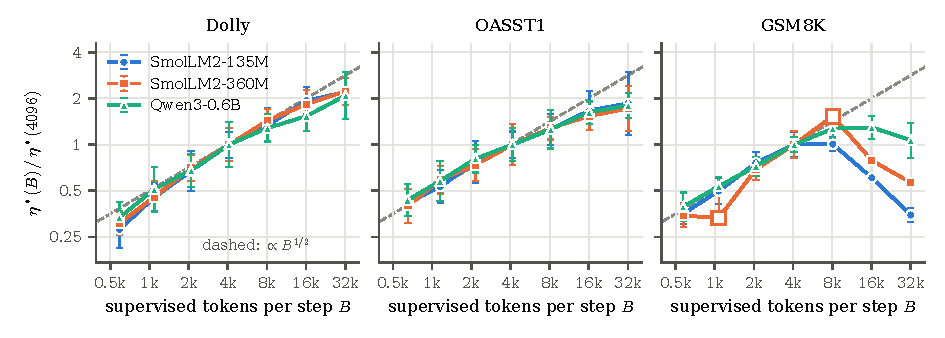
\includegraphics[width=\textwidth]{figures/lr_star.pdf}
\caption{Optimal learning rate $\eta^*(B)$ relative to $\eta^*(4{,}096)$, with 68\% intervals, against the realised number of supervised tokens per step (tick labels use k $=1{,}024$). The dashed line has slope $1/2$. Open markers are columns flagged because the best learning rate is next to one that diverged in one seed.}
\label{fig:lrstar}
\end{figure}

\begin{table}[t]
\centering
\caption{Learning rate and fixed-data critical batch size (CBS) in the nine settings. $\alpha$: exponent of $\eta^*(B)$ over all unflagged columns, with its 68\% interval (pre-registered); $\alpha_{\le 4\mathrm{k}}$ and $\alpha_{\ge 4\mathrm{k}}$: the same fit over $B \le 4{,}096$ and $B \ge 4{,}096$ (descriptive); peak: the batch size with the largest $\eta^*$ where this is not the largest batch, with the exponent fitted up to it. CBS in supervised tokens per step at $\epsilon = 0.005$ and $0.01$; $^{\ast}$: at the top of the grid, so a lower bound. Steps: optimizer steps in one epoch at the CBS. $\Delta L_{32\mathrm{k}}$: held-out loss at $B=32{,}768$ minus the lowest loss over all $B$, in nats.}
\label{tab:main}
\footnotesize
\setlength{\tabcolsep}{3.5pt}
\begin{tabular}{llcrrrrrrrr}
\toprule
model & corpus & $\alpha$ [68\% interval] & $\alpha_{\le 4\mathrm{k}}$ & $\alpha_{\ge 4\mathrm{k}}$ & peak & \begin{tabular}[b]{@{}r@{}}$\alpha$ to\\ peak\end{tabular} & CBS & CBS$_{0.01}$ & steps & $\Delta L_{32\mathrm{k}}$ \\
\midrule
SmolLM2-135M & Dolly & 0.51 [0.47, 0.55] & 0.65 & 0.40 & -- & -- & 16,384 & 32,768 & 66 & 0.009 \\
SmolLM2-135M & OASST1 & 0.41 [0.37, 0.47] & 0.48 & 0.33 & -- & -- & 8,192 & 16,384 & 78 & 0.014 \\
SmolLM2-135M & GSM8K & 0.00 [$-$0.02, 0.02] & 0.54 & $-$0.56 & 8,192 & 0.40 & 2,048 & 4,096 & 396 & 0.146 \\
\midrule
SmolLM2-360M & Dolly & 0.51 [0.47, 0.53] & 0.62 & 0.38 & -- & -- & 16,384 & 32,768 & 66 & 0.007 \\
SmolLM2-360M & OASST1 & 0.38 [0.33, 0.42] & 0.48 & 0.27 & -- & -- & 8,192 & 32,768 & 78 & 0.010 \\
SmolLM2-360M & GSM8K & 0.01 [$-$0.01, 0.03] & 0.54 & $-$0.32 & 8,192 & 0.54 & 4,096 & 4,096 & 198 & 0.074 \\
\midrule
Qwen3-0.6B & Dolly & 0.45 [0.41, 0.50] & 0.56 & 0.34 & -- & -- & 16,384 & 32,768 & 64 & 0.007 \\
Qwen3-0.6B & OASST1 & 0.36 [0.32, 0.39] & 0.46 & 0.29 & -- & -- & 32,768$^{\ast}$ & 32,768 & 19 & 0.004 \\
Qwen3-0.6B & GSM8K & 0.30 [0.27, 0.33] & 0.47 & 0.07 & 16,384 & 0.38 & 8,192 & 8,192 & 97 & 0.021 \\

\end{tabular}
\end{table}

These results bear on H1 and H1b as follows. $\eta^*$ is not flat in any setting: from $B = 512$ to its largest value it rises by a factor of 2.8 to 7.9. It then flattens on Dolly and OASST1 and falls on GSM8K, so H1 is not falsified. H1b fails. The run-averaged $\bsimple$ is below 32,768 tokens in all nine settings (Section~\ref{sec:noise-results}), so H1b predicts a peak within a factor of 2 of it in every setting. Only the three GSM8K settings have a peak, and it lies 8, 13 and 23 times above the run average, beyond the factor of 4 that falsifies the hypothesis.

\subsection{Fixed-data critical batch size}\label{sec:fixed}

Figure~\ref{fig:lossgap} shows the held-out loss at $\eta^*(B)$ relative to the best batch size. On Dolly and OASST1 the loss is flat to within 0.005 nats up to at least 8,192 tokens and is only 0.004 to 0.014 nats above its best value at 32,768. On GSM8K it begins to rise between 4,096 and 16,384 tokens, depending on the model, and is 0.021 to 0.146 nats above its best value at 32,768. The fixed-data critical batch size (Table~\ref{tab:main}) is 16,384 tokens on Dolly for all three models, 8,192 on OASST1 for the SmolLM2 models and at least 32,768 for Qwen3-0.6B, and 2,048, 4,096 and 8,192 on GSM8K. With the looser threshold of 0.01 nats the values rise by at most a factor of 4. In examples, these batch sizes correspond to about 210 examples per step on Dolly, 36 on OASST1 for the SmolLM2 models, and 16 to 67 on GSM8K. At the critical batch size one epoch takes 64 to 78 optimizer steps on Dolly and on OASST1 with the SmolLM2 models, and 97 to 396 steps on GSM8K.

\begin{figure}[t]
\centering
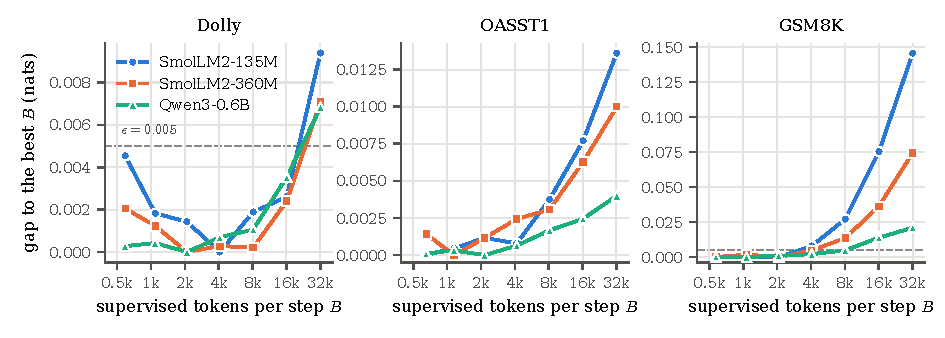
\includegraphics[width=\textwidth]{figures/loss_gap.pdf}
\caption{Held-out loss at $\eta^*(B)$ minus the lowest such loss over $B$, in nats. The dashed line marks $\epsilon = 0.005$. The vertical scales differ between panels. Tick labels use k $=1{,}024$.}
\label{fig:lossgap}
\end{figure}

For H4, the critical batch size on Dolly is the same for all three models, as the hypothesis predicts. On OASST1 it is 8,192, 8,192 and at least 32,768, a change of more than a factor of 2 that does not count as a size effect under the pre-registered rule, because the SmolLM2-135M to SmolLM2-360M pair does not move. On GSM8K it doubles at each step of the ladder, 2,048, 4,096 and 8,192, and here the pair within one family moves. The prediction of invariance therefore holds on one corpus, not the required two, while the falsification condition, a counted size effect on two corpora, is met on one. By its own criteria H4 is neither supported nor falsified.

\subsection{The gradient noise scale is small at the start and grows quickly}\label{sec:noise-results}

Table~\ref{tab:noise} and Figure~\ref{fig:noise} give $\bsimple$ along the epoch. At the first step it is between 300 and 8,800 tokens, below 8,192 in eight of the nine settings, so the step-zero prediction of H2 is falsified. It then rises steeply: after a quarter of the epoch it is 3.8 to 88 times its initial value, and at the end of the epoch it is 2.2 to 61 times larger than at the start, which is the growth that H2 predicted. The two terms of the estimate show where the rise comes from. Between the first step and the 25\% point, $|G|^2$ falls by a factor of 5.6 to 298, while $\mathrm{tr}(\Sigma)$ falls only by a factor of 1.2 to 3.4. At the start of fine-tuning the examples of a corpus therefore share a large common gradient, and once that component has been learned what remains is mostly specific to each example. A likely cause is that the pretrained model first has to adapt to the prompt template, the style of the responses and where they end, which all examples have in common. GSM8K, whose solutions share a rigid format, has the smallest initial noise scale in every model. The first version of H2, written before the freeze, predicted a small noise scale at the start for a similar reason; it was reversed on the strength of a single smoke-run measurement, taken with an early estimator that had the same flaw as the first version described in Appendix~\ref{app:deviations}, item 2.

\begin{table}[t]
\centering
\caption{Simple noise scale $\bsimple$ (supervised tokens; k $=1{,}000$) at five points of a one-epoch run at $B = 4{,}096$ and $\eta^*(4{,}096)$. Run average: mean $\mathrm{tr}(\Sigma)$ over the five points divided by mean $|G|^2$ (pre-registered). 25--100\%: the same average without the first point (exploratory). The last column repeats the fixed-data CBS from Table~\ref{tab:main}.}
\label{tab:noise}
\small
\begin{tabular}{llrrrrrrrr}
\toprule
model & corpus & 0\% & 25\% & 50\% & 75\% & 100\% & run average & 25--100\% & CBS \\
\midrule
SmolLM2-135M & Dolly & 3.0k & 72k & 39k & 41k & 41k & 8.5k & 46k & 16,384 \\
SmolLM2-135M & OASST1 & 5.2k & 31k & 41k & 18k & 19k & 13k & 25k & 8,192 \\
SmolLM2-135M & GSM8K & 0.3k & 7.3k & 11k & 14k & 18k & 0.6k & 11k & 2,048 \\
\midrule
SmolLM2-360M & Dolly & 2.8k & 76k & 62k & 50k & 52k & 7.9k & 57k & 16,384 \\
SmolLM2-360M & OASST1 & 7.3k & 28k & 37k & 13k & 16k & 13k & 20k & 8,192 \\
SmolLM2-360M & GSM8K & 0.5k & 13k & 9.7k & 17k & 20k & 1.0k & 13k & 4,096 \\
\midrule
Qwen3-0.6B & Dolly & 4.0k & 148k & 121k & 104k & 71k & 9.6k & 105k & 16,384 \\
Qwen3-0.6B & OASST1 & 8.8k & 367k & 73k & 68k & 95k & 28k & 98k & 32,768 \\
Qwen3-0.6B & GSM8K & 0.4k & 34k & 22k & 15k & 13k & 0.7k & 20k & 8,192 \\
\bottomrule

\end{tabular}
\end{table}

\begin{figure}[t]
\centering
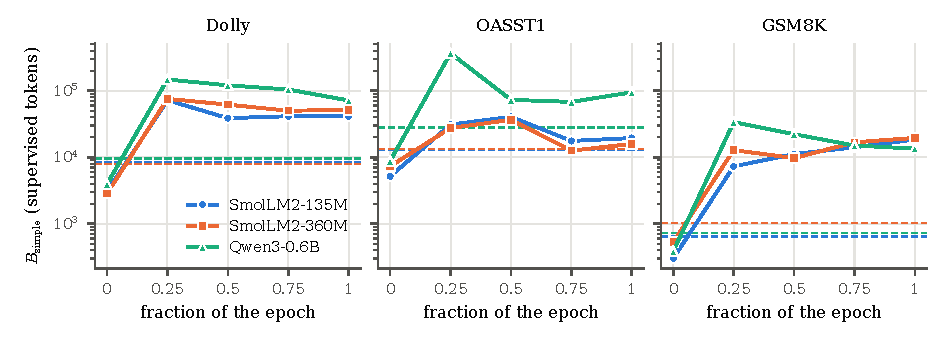
\includegraphics[width=\textwidth]{figures/noise.pdf}
\caption{Simple noise scale along the epoch. Dashed lines show each setting's run average, which lies close to the first-step value because the first step dominates the mean of $|G|^2$.}
\label{fig:noise}
\end{figure}

This shape determines how well the pre-registered predictor can work. The run average divides the mean of $\mathrm{tr}(\Sigma)$ by the mean of $|G|^2$, and the mean of $|G|^2$ is dominated by the first point, so the run average stays within a factor of about 3 of the first-step value and far below the noise scale over most of the epoch. Against the fixed-data critical batch size its Spearman correlation is 0.62 and its median ratio is 0.52, with five of the nine settings within a factor of 2 and ratios ranging from 0.09 to 1.62. This lies between the support and falsification thresholds of H3 (a correlation of at least 0.7 for support and below 0.4 for falsification, with the median ratio barely inside $[0.5, 2]$), so H3 is inconclusive.

The following analysis was not planned and was done after the results above had been seen. Leaving out the first point, the average over the 25\% to 100\% points has a Spearman correlation of 0.93 with the fixed-data critical batch size, but it is 2.4 to 6.4 times larger (median 3.0), so none of the nine settings is within a factor of 2. It also places the three GSM8K peaks of $\eta^*$ at 0.62 to 0.83 of the noise scale, within the factor of 2 that H1b asked for, and it is above 32,768 for all three models on Dolly, where no peak appears. With the SmolLM2 models on OASST1 it predicts a peak near 20,000 to 25,000 tokens, where $\eta^*$ instead keeps rising slowly. These observations suggest that a noise scale measured after the first part of the run behaves much as Li et al.~\cite{li2024surge} predict, but they come from the same data that motivated them and need a separate test. Section~\ref{sec:confirm} reports one.

\subsection{Branched critical batch size}\label{sec:branched}

Table~\ref{tab:branched} and Figure~\ref{fig:branched} show the branched critical batch size. In all three settings it is smallest at the 0\% point, where branches start from the pretrained model with a fresh optimizer: 8,192 tokens on Dolly for both models and 1,024 on GSM8K. Later in the epoch it is at least 32,768 on Dolly (except for SmolLM2-135M at the 25\% point, at 8,192) and 4,096 on GSM8K. The shorter window of 12.5\% gives the same value on Dolly and a smaller one on GSM8K (2,048 against 4,096). The extra learning rates added at the edges of the branch sweeps changed only one of the 15 values: SmolLM2-135M with Dolly at the 50\% point moves from 16,384 with the planned three-point sweep to at least 32,768. In pretraining, Merrill et al.~\cite{merrill2025} found a critical batch size that starts near zero and grows during training, and SFT shows the same pattern over a single epoch.

\begin{table}[t]
\centering
\caption{Branched critical batch size (supervised tokens per step) by checkpoint and window $\Delta$ (fraction of the epoch). 3-lr: the planned sweep of three learning rates, $\epsilon = 0.005$; bracketed: with the extra learning rates added at sweep edges, at $\epsilon = 0.005$ and $0.01$. $^{\ast}$: at the top of the grid, so a lower bound. Fixed-data: the CBS of Table~\ref{tab:main}. $\bsimple(t)$: noise scale at the same fraction of the noise run (k $=1{,}000$; exploratory comparison).}
\label{tab:branched}
\footnotesize
\setlength{\tabcolsep}{4pt}
\begin{tabular}{lrrrrrrr}
\toprule
 & & & & \multicolumn{2}{c}{bracketed} & & \\
\cmidrule(lr){5-6}
setting & checkpoint & $\Delta$ & 3-lr & $\epsilon=0.005$ & $\epsilon=0.01$ & fixed-data & $\bsimple(t)$ \\
\midrule
SmolLM2-135M, Dolly & 0\% & 25\% & 8,192 & 8,192 & 8,192 & 16,384 & 3.0k \\
 & 25\% & 25\% & 8,192 & 8,192 & 32,768$^{\ast}$ & 16,384 & 72k \\
 & 50\% & 25\% & 16,384 & 32,768$^{\ast}$ & 32,768$^{\ast}$ & 16,384 & 39k \\
 & 50\% & 12.5\% & 32,768$^{\ast}$ & 32,768$^{\ast}$ & 32,768$^{\ast}$ & 16,384 & 39k \\
 & 75\% & 25\% & 32,768$^{\ast}$ & 32,768$^{\ast}$ & 32,768$^{\ast}$ & 16,384 & 41k \\
\midrule
SmolLM2-360M, Dolly & 0\% & 25\% & 8,192 & 8,192 & 16,384 & 16,384 & 2.8k \\
 & 25\% & 25\% & 32,768$^{\ast}$ & 32,768$^{\ast}$ & 32,768$^{\ast}$ & 16,384 & 76k \\
 & 50\% & 25\% & 32,768$^{\ast}$ & 32,768$^{\ast}$ & 32,768$^{\ast}$ & 16,384 & 62k \\
 & 50\% & 12.5\% & 32,768$^{\ast}$ & 32,768$^{\ast}$ & 32,768$^{\ast}$ & 16,384 & 62k \\
 & 75\% & 25\% & 32,768$^{\ast}$ & 32,768$^{\ast}$ & 32,768$^{\ast}$ & 16,384 & 50k \\
\midrule
SmolLM2-135M, GSM8K & 0\% & 25\% & 1,024 & 1,024 & 2,048 & 2,048 & 0.3k \\
 & 25\% & 25\% & 4,096 & 4,096 & 4,096 & 2,048 & 7.3k \\
 & 50\% & 25\% & 4,096 & 4,096 & 4,096 & 2,048 & 11k \\
 & 50\% & 12.5\% & 2,048 & 2,048 & 4,096 & 2,048 & 11k \\
 & 75\% & 25\% & 4,096 & 4,096 & 4,096 & 2,048 & 14k \\
\bottomrule

\end{tabular}
\end{table}

\begin{figure}[t]
\centering
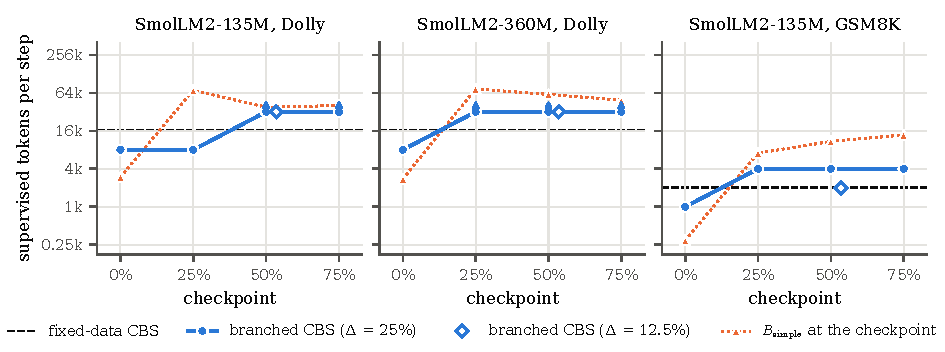
\includegraphics[width=\textwidth]{figures/branched.pdf}
\caption{Branched critical batch size against the checkpoint (bracketed sweeps, $\epsilon = 0.005$). Arrows mark values at the top of the grid, which are lower bounds. The dashed line is the fixed-data CBS of the same setting. The dotted line is the noise scale measured at the same fraction of the epoch in the noise run, an exploratory comparison; that run uses $B = 4{,}096$, whereas the branched base run uses $B = 1{,}024$.}
\label{fig:branched}
\end{figure}

H2b was scored as follows. The plan does not say which checkpoint should be compared with the fixed-data critical batch size, and this was decided after both tables had been seen (Appendix~\ref{app:deviations}, item 8). We therefore report every checkpoint and treat the warm checkpoints, at 25\% to 75\%, as the test of the mechanism H2b names, the start-up cost that a run from the pretrained model pays and a branch from a warm checkpoint does not. On GSM8K the branched value is within a factor of 2 of the fixed-data value of 2,048 at every checkpoint, which falsifies H2b in that setting. On Dolly the warm branched values are at least 32,768, at least twice the fixed-data value of 16,384, but because they sit at the top of the grid the size of the gap cannot be measured, and extending the grid is not meaningful: a 25\% window at 65,536 tokens per step would be about four steps. At the 0\% point the branched value is half the fixed-data value in all three settings, the opposite of the predicted direction, and the gap is not larger on the smaller corpus, as predicted, since GSM8K has fewer tokens than Dolly but the smaller gap. We conclude that H2b is not supported: it is falsified in one setting and cannot be decided in the other two.

H3 named the fixed-data critical batch size, so the branched values do not test it; three settings are also too few for a rank correlation. For completeness, the branched value at the 0\% point is within a factor of 2 of the run-averaged noise scale in all three settings (ratios 0.96, 1.04 and 1.6), and at the warm checkpoints it is between 1.0 and 6.4 times the run average. As an exploratory comparison at matching times, the branched value at the 0\% point is about three times the first-step noise scale (2.7 to 3.4) in all three settings, and at the warm checkpoints it is 0.1 to 0.9 times the noise scale measured at the same point, with the Dolly values being lower bounds. Both quantities grow during the epoch, the noise scale more steeply.

\subsection{Controls}\label{sec:controls}

Table~\ref{tab:controls} gives the two controls in the pilot setting. Holding the $\beta_2$ half-life fixed in tokens multiplies $\eta^*$ by 1.25 at $B = 512$ and by 0.84 at $32{,}768$, so it moves by less than the factor of 1.3 that H5 set, and H5 is supported. The direction of both changes is the one Marek et al.~\cite{marek2025} describe, a flatter $\eta^*(B)$, but the size is much smaller: the exponent between the two extreme batch sizes falls from 0.48 to 0.38, against the drop to about 0.16 that their pretraining result implies. The control also lowers the held-out loss at $B = 512$ by 0.002 nats, below $\epsilon$, and leaves it unchanged at $32{,}768$. Clipping the gradient at 1.0 changes $\eta^*$ by a factor of 1.01 at both ends and the loss by less than 0.001 nats.

\begin{table}[t]
\centering
\caption{$\beta_2$ and clipping controls in the pilot setting (SmolLM2-360M, Dolly), three seeds. Ratio: $\eta^*$ of the control divided by $\eta^*$ of the main grid.}
\label{tab:controls}
\small
\begin{tabular}{rlccrr}
\toprule
$B$ & variant & $\eta^*$ & 68\% interval & loss at $\eta^*$ & ratio \\
\midrule
512 & main grid ($\beta_2 = 0.95$, no clipping) & $1.58\mathrm{e}{-5}$ & [$1.3\mathrm{e}{-5}$, $1.9\mathrm{e}{-5}$] & 1.9124 & -- \\
 & $\beta_2$ half-life fixed in tokens & $1.96\mathrm{e}{-5}$ & [$1.6\mathrm{e}{-5}$, $2.4\mathrm{e}{-5}$] & 1.9103 & 1.25 \\
 & gradient clipping at 1.0 & $1.58\mathrm{e}{-5}$ & [$1.3\mathrm{e}{-5}$, $1.9\mathrm{e}{-5}$] & 1.9122 & 1.01 \\
\midrule
32,768 & main grid ($\beta_2 = 0.95$, no clipping) & $1.14\mathrm{e}{-4}$ & [$9.3\mathrm{e}{-5}$, $1.4\mathrm{e}{-4}$] & 1.9174 & -- \\
 & $\beta_2$ half-life fixed in tokens & $9.57\mathrm{e}{-5}$ & [$9.0\mathrm{e}{-5}$, $1.0\mathrm{e}{-4}$] & 1.9174 & 0.84 \\
 & gradient clipping at 1.0 & $1.15\mathrm{e}{-4}$ & [$1.1\mathrm{e}{-4}$, $1.2\mathrm{e}{-4}$] & 1.9166 & 1.01 \\
\bottomrule

\end{tabular}
\end{table}

The 8-bit optimizer stack used for Qwen3-0.6B was compared with standard AdamW on the full SmolLM2-135M grid for Dolly (Table~\ref{tab:8bit}). The two values of $\eta^*$ differ by a factor of 0.85 to 1.00, and their intervals overlap at every batch size, which meets the test set in the plan. The exponent is 0.55 [0.52, 0.59] against 0.51 [0.47, 0.55], and the critical batch size is the same, 16,384 at $\epsilon = 0.005$ and 32,768 at $\epsilon = 0.01$. The 8-bit optimizer raises the loss at $B = 512$ by 0.002 nats, an effect that shrinks as the number of steps falls and is negligible from $B = 4{,}096$ upwards. The Qwen3-0.6B results are therefore not confounded with the optimizer stack, at least as far as this test can show.

\begin{table}[t]
\centering
\caption{Optimizer-stack control: SmolLM2-135M on Dolly with AdamW (main grid) and with the configuration used for Qwen3-0.6B (8-bit AdamW, gradient checkpointing, smaller micro-batches), at the same learning rates and seeds. $\Delta L$: loss of the 8-bit run minus that of the main run at $\eta^*$, in thousandths of a nat.}
\label{tab:8bit}
\small
\begin{tabular}{rccccrr}
\toprule
 & \multicolumn{2}{c}{AdamW} & \multicolumn{2}{c}{8-bit AdamW} & & \\
\cmidrule(lr){2-3}\cmidrule(lr){4-5}
$B$ & $\eta^*$ & 68\% interval & $\eta^*$ & 68\% interval & ratio & $\Delta L$ \\
\midrule
512 & $2.17\mathrm{e}{-5}$ & [$1.6\mathrm{e}{-5}$, $2.9\mathrm{e}{-5}$] & $1.84\mathrm{e}{-5}$ & [$1.5\mathrm{e}{-5}$, $2.3\mathrm{e}{-5}$] & 0.85 & +2.0 \\
1,024 & $3.50\mathrm{e}{-5}$ & [$2.8\mathrm{e}{-5}$, $4.3\mathrm{e}{-5}$] & $3.29\mathrm{e}{-5}$ & [$2.7\mathrm{e}{-5}$, $4.0\mathrm{e}{-5}$] & 0.94 & +1.0 \\
2,048 & $5.21\mathrm{e}{-5}$ & [$3.9\mathrm{e}{-5}$, $7.0\mathrm{e}{-5}$] & $4.94\mathrm{e}{-5}$ & [$3.7\mathrm{e}{-5}$, $6.6\mathrm{e}{-5}$] & 0.95 & +0.5 \\
4,096 & $7.74\mathrm{e}{-5}$ & [$6.4\mathrm{e}{-5}$, $9.4\mathrm{e}{-5}$] & $7.63\mathrm{e}{-5}$ & [$6.3\mathrm{e}{-5}$, $9.3\mathrm{e}{-5}$] & 0.99 & +0.1 \\
8,192 & $1.03\mathrm{e}{-4}$ & [$8.0\mathrm{e}{-5}$, $1.3\mathrm{e}{-4}$] & $1.03\mathrm{e}{-4}$ & [$7.9\mathrm{e}{-5}$, $1.3\mathrm{e}{-4}$] & 0.99 & 0.0 \\
16,384 & $1.49\mathrm{e}{-4}$ & [$1.2\mathrm{e}{-4}$, $1.8\mathrm{e}{-4}$] & $1.49\mathrm{e}{-4}$ & [$1.2\mathrm{e}{-4}$, $1.8\mathrm{e}{-4}$] & 1.00 & 0.0 \\
32,768 & $1.71\mathrm{e}{-4}$ & [$1.4\mathrm{e}{-4}$, $2.1\mathrm{e}{-4}$] & $1.71\mathrm{e}{-4}$ & [$1.4\mathrm{e}{-4}$, $2.1\mathrm{e}{-4}$] & 1.00 & $-$0.1 \\
\bottomrule

\end{tabular}
\end{table}

\subsection{Retuning the learning rate and the other corpora}\label{sec:transfer}

H6 asks whether the gain from retuning the learning rate for a new batch size carries over to data the model was not trained on. The measurement was fixed before any cross-corpus loss had been read (Appendix~\ref{app:deviations}, item 8). For each setting and each batch size other than 4,096, the reference learning rate is the grid point nearest $\eta^*(4{,}096)$, which is what a practitioner would keep when changing only the batch size, and the retuned learning rate is the grid point with the lowest held-out loss on the fine-tuning corpus at that batch size (seed 1). The gain on a corpus is its held-out loss at the reference learning rate minus its loss at the retuned one.

Of the 54 pairs of setting and batch size, the retuned learning rate differs from the reference in 33. It is lower in 20 cases, at batch sizes up to 2,048 and, for SmolLM2-135M on GSM8K, also at 16,384 and 32,768, past the peak of $\eta^*$; it is higher in 13 cases, all at 8,192 or more. Figure~\ref{fig:transfer} shows the gains. The same-corpus gain is non-negative by construction. When retuning lowers the learning rate, the loss on the other two corpora also improves, in all 40 cases, and usually by more than on the fine-tuning corpus itself; where the same-corpus gain is at least 0.005 nats, the median ratio of cross-corpus to same-corpus gain is 8.7. When retuning raises the learning rate, the other corpora get worse in 22 of 26 cases, by up to 0.126 nats, while the gain on the fine-tuning corpus is at most 0.007 nats. Taken together, at a given batch size the lower of the two learning rates gives the lower loss on the other corpora in 62 of 66 comparisons, whichever of the two is better for the fine-tuning corpus. A higher learning rate moves the model further from its pretrained state, which raises its loss on other data, in line with the larger forgetting of full fine-tuning reported by Biderman et al.~\cite{biderman2024}. The effect is largest for models fine-tuned on GSM8K, where at $B = 512$ the retuned learning rate lowers the loss on Dolly and OASST1 by 0.22 to 0.77 nats.

\begin{figure}[t]
\centering
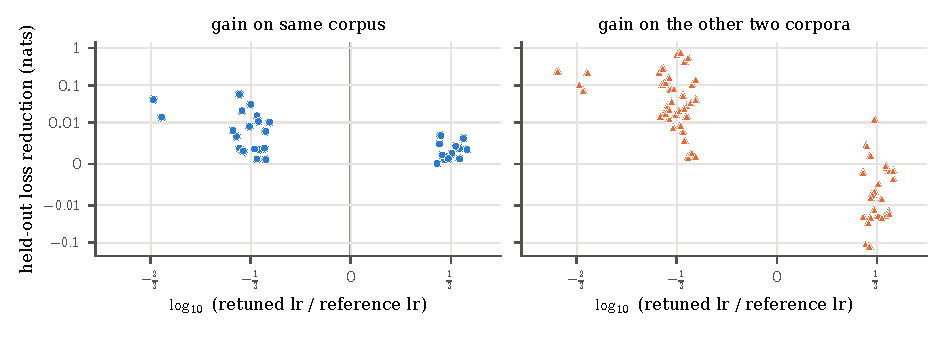
\includegraphics[width=\textwidth]{figures/transfer.pdf}
\caption{Gain in held-out loss from retuning the learning rate for the batch size, against the size of the change (decades), for the 33 cases where the retuned learning rate differs from the reference. Left: the fine-tuning corpus; right: the other two corpora. The vertical axis is linear between $-0.01$ and $0.01$ and logarithmic outside. Points are spread slightly along the horizontal axis to reduce overlap.}
\label{fig:transfer}
\end{figure}

\subsection{Summary of the hypotheses}

Table~\ref{tab:verdicts} collects the outcome for each hypothesis.

\begin{table}[t]
\centering
\caption{Pre-registered hypotheses and outcomes.}
\label{tab:verdicts}
\small
\begin{tabular}{lp{0.62\textwidth}l}
\toprule
 & result & outcome \\
\midrule
H1 & $\eta^*$ rises 2.8 to 7.9 times, then flattens (Dolly, OASST1) or falls (GSM8K) & not falsified \\
H1b & all run averages are below 32,768, but only GSM8K has a peak, 8 to 23 times above the run average & falsified \\
H2 & first-step $\bsimple$ below 8,192 in 8 of 9 settings; it rises 2.2 to 61 times by the end of the epoch & falsified \\
H2b & within a factor of 2 on GSM8K at every checkpoint; Dolly censored at the warm checkpoints; at 0\% the branched value is half the fixed-data value & not supported \\
H3 & Spearman 0.62, median ratio 0.52, 5 of 9 within a factor of 2 & inconclusive \\
H4 & invariant on Dolly; 4-fold change on OASST1 (not a size effect by the rule) and on GSM8K (a size effect) & inconclusive \\
H5 & $\eta^*$ moves 1.25 times at $B=512$ and 1.19 times at $32{,}768$ & supported \\
H6 & lowering $\eta$ helps the other corpora (40 of 40); raising it hurts them (22 of 26) & measured \\
\bottomrule
\end{tabular}
\end{table}

\section{Confirmatory study}\label{sec:confirm}

The analysis at the end of Section~\ref{sec:noise-results} found that the noise scale measured after the first quarter of the epoch tracks the fixed-data critical batch size and the location of the peak of $\eta^*$, but it was found in the same nine settings it describes. We therefore tested it on new data in a second pre-registered study. Its design and predictions were written on 9 November 2026, after every result above had been seen and before any run of the study existed, and were committed under the tag \texttt{prereg-confirm-v1} and pushed to GitHub on the same day. The first run of the study was queued two days later. GitHub records the time of the push, but the repository is private until publication, so this record is not yet public. Once the runs had started, every configuration was written and queued by the same scripts as in the main study, and nothing was decided by hand. There were no departures from the plan.

\subsection{Design and predictions}

In this section $\blate$ denotes the noise scale of a noise run averaged over its 25\%, 50\%, 75\% and 100\% points: the mean of $\mathrm{tr}(\Sigma)$ over these four points divided by the mean of $|G|^2$ over them. It is the 25--100\% column of Table~\ref{tab:noise}. The study has two parts.

The first part adds three corpora, each trained with SmolLM2-135M. They were chosen for tasks that the main study does not cover and for sizes close to its range: Alpaca-8k, a fixed random sample of 8,000 examples from the cleaned release of the Alpaca data~\cite{taori2023alpaca}, which consists of synthetic general instructions; CodeAlpaca~\cite{chaudhary2023codealpaca}, about 20,000 instructions about code; and the training split of DialogSum~\cite{chen2021dialogsum}, in which the response is a summary of a dialogue. They have 7,000, 19,016 and 11,448 training examples and 1.01M, 1.20M and 0.41M supervised tokens per epoch. DialogSum is smaller than any main corpus, and at $B = 32{,}768$ one epoch of it is 12 steps. Formatting, held-out sets, truncation and training follow Section~\ref{sec:setup}. Each setting went through the main-grid procedure unchanged: the $B = 4{,}096$ column over two decades, the seven-by-seven grid centred by the square-root rule, three seeds at the best point of each column and its two neighbours, and one noise run at $B = 4{,}096$ and $\eta^*(4{,}096)$ with measurements at 0, 25, 50, 75 and 100\% of the epoch. Because a software restriction on the GPU machine blocked the library used to download the corpora, all corpora were read in this study from files exported by the same code on another machine; for the three main corpora these files reproduce the splits of the main study exactly.

The second part repeats the noise run of each of the nine original settings with a new seed (seed 2, or seed 3 for SmolLM2-360M with Dolly, which already had two), at the same batch size and learning rate, with measurements at 0, 2, 5, 10, 25, 50, 75 and 100\% of the epoch.

The predictions, as fixed in the plan, were the following.
\begin{description}
\item[C1 (critical batch size from the late noise scale).] In each new setting the fixed-data critical batch size lies within a factor of 2 of $\blate/3$, that is, in $[\blate/6, \blate/1.5]$. A critical batch size at the top of the grid counts as consistent if $\blate/1.5 \ge 32{,}768$. Supported if this holds in all three new settings, falsified if it fails in two or more. In the nine original settings it holds in eight.
\item[C2 (peak).] If $\blate \le 16{,}384$, $\eta^*(B)$ has an interior peak, that is, its largest value is at a batch size below 32,768, and this batch size is within a factor of 2 of $\blate$. If $\blate \ge 65{,}536$, there is no interior peak. Between these values no prediction is made. Falsified if it fails in any new setting where it applies. It holds wherever it applies in the original settings.
\item[C3 (square-root rule).] The exponent fitted over the columns with $B \le 4{,}096$ lies in $[0.40, 0.70]$ in each new setting. Falsified if it fails in two or more. In the original settings it ranged from 0.46 to 0.65.
\item[C4 (replication).] With the new noise runs of the nine original settings: (a) $\blate$ is within a factor of 2 of its original value in at least 8 of the 9 settings; (b) $\bsimple$ at the 25\% point is at least 4 times its first-step value in at least 7 of 9; (c) $|G|^2$ at the 5\% point is at most a fifth of its first-step value in at least 7 of 9, which tests whether the mean gradient collapses during or just after warmup; (d) C1, computed with the new $\blate$ and the existing fixed-data critical batch size, holds in at least 7 of 9.
\end{description}

\subsection{Results on the new corpora}

\begin{table}[t]
\centering
\caption{Predictions C1 to C3 on the three new corpora (SmolLM2-135M). $\blate$: late noise scale in supervised tokens (k $=1{,}000$). Interval: $[\blate/6, \blate/1.5]$, the range predicted by C1 for the fixed-data CBS. Peak: the batch size with the largest $\eta^*$, if it is below 32,768. C2 applies only where $\blate \le 16{,}384$ or $\blate \ge 65{,}536$. $\alpha_{\le 4\mathrm{k}}$: exponent over $B \le 4{,}096$ with its 68\% interval; C3 requires it to lie in $[0.40, 0.70]$.}
\label{tab:confirm-new}
\small
\setlength{\tabcolsep}{4pt}
\begin{tabular}{lrcrcrclc}
\toprule
corpus & $\blate$ & interval & CBS & C1 & peak & C2 & $\alpha_{\le 4\mathrm{k}}$ & C3 \\
\midrule
Alpaca-8k & 32k & [5.3k, 21k] & 8,192 & yes & none & -- & 0.56 [0.47, 0.65] & yes \\
CodeAlpaca & 28k & [4.6k, 19k] & 8,192 & yes & none & -- & 0.63 [0.56, 0.70] & yes \\
DialogSum & 6.1k & [1.0k, 4.1k] & 1,024 & yes & 4,096 & yes & 0.44 [0.39, 0.49] & yes \\
\bottomrule

\end{tabular}
\end{table}

\begin{figure}[t]
\centering
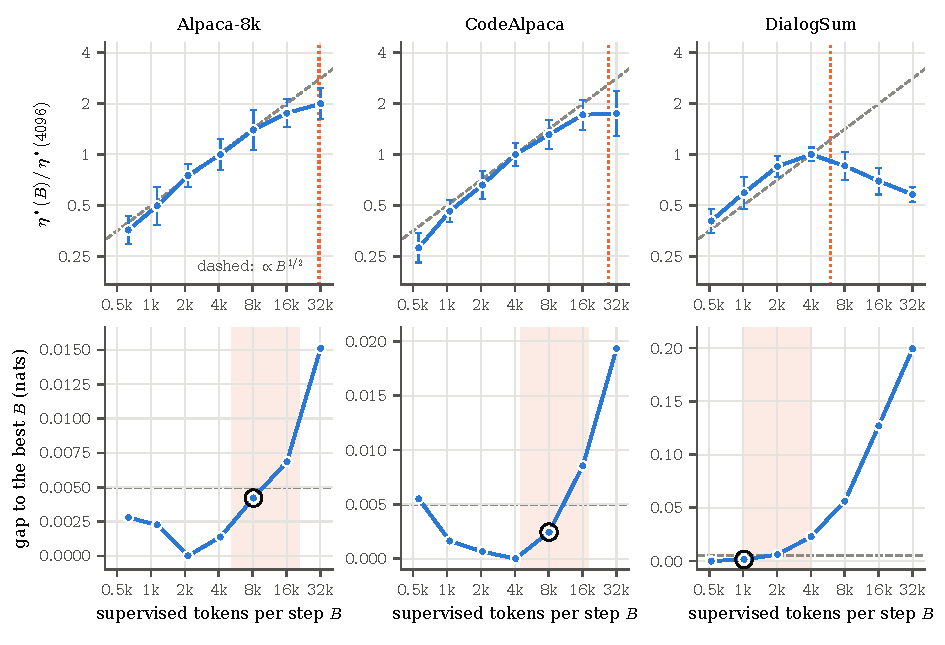
\includegraphics[width=\textwidth]{figures/confirm.pdf}
\caption{The three new corpora. Top: $\eta^*(B)/\eta^*(4{,}096)$ with 68\% intervals; dashed, the square-root rule; dotted, $\blate$. Bottom: held-out loss at $\eta^*(B)$ minus the lowest such loss, with $\epsilon = 0.005$ dashed. The shaded band is the interval that C1 predicts for the fixed-data CBS, and the circled point is the measured CBS. The vertical scales of the lower panels differ. Tick labels use k $=1{,}024$.}
\label{fig:confirm}
\end{figure}

The three new grids contain 276 runs. One diverged (DialogSum at $B = 8{,}192$ and the largest learning rate of its column), no column needed an extension, and at the best learning rate of each column at most 0.06\% of the steps were skipped by the loss scaler. Table~\ref{tab:confirm-new} and Figure~\ref{fig:confirm} give the results.

The fixed-data critical batch size is 8,192 tokens on Alpaca-8k and CodeAlpaca and 1,024 on DialogSum. All three lie inside their predicted intervals, so C1 is supported. The ratio of $\blate$ to the critical batch size is 3.9, 3.4 and 6.0, within the range of 2.4 to 6.4 found in the main study. The DialogSum result is close to the edge in two ways: its interval begins at 1,019 tokens, and its critical batch size stops at 1,024 because the loss at 2,048 is 0.0061 nats above the loss at 512, just over $\epsilon$. With $\epsilon = 0.01$ the three critical batch sizes are 16,384, 16,384 and 2,048, which also lie inside the intervals.

C2 applies only to DialogSum, the one new setting with $\blate$ below 16,384 (about 6,100 tokens). Its $\eta^*$ peaks at $B = 4{,}096$, at 0.67 of $\blate$, and falls by a factor of 1.7 from there to 32,768, so C2 holds where it applies; the GSM8K peaks of the main study lie at 0.62 to 0.83 of $\blate$. On Alpaca-8k and CodeAlpaca, $\blate$ is about 32,000 and 28,000 tokens, in the range where the plan makes no prediction. On both corpora $\eta^*$ rises across the whole grid, by factors of 5.6 and 6.3 between 512 and 32,768, and the rise slows above 8,192 tokens; on CodeAlpaca $\eta^*$ is almost the same at 16,384 and 32,768.

The exponent below 4,096 tokens is 0.56, 0.63 and 0.44, inside $[0.40, 0.70]$ in all three settings, so C3 is not falsified. The DialogSum value is close to the lower bound, and its interval extends below it.

The noise scale has the same shape along the epoch as in the main study. Between the first step and the 25\% point, $|G|^2$ falls by a factor of 27 to 82 on the new corpora while $\mathrm{tr}(\Sigma)$ falls by a factor of 1.4 to 2.6, and $\bsimple$ at the first step is between 110 and 3,300 tokens. DialogSum also has the largest loss penalty at large batches of any setting in this paper, 0.20 nats above its best value at $B = 32{,}768$, against at most 0.15 nats on GSM8K.

\subsection{Replication of the noise runs}

\begin{table}[t]
\centering
\caption{Repeated noise runs for the nine original settings (C4). $\blate$ of the original seed-1 run and of the new run, in supervised tokens (k $=1{,}000$); for SmolLM2-360M with Dolly the original value is that of seed 1, while Table~\ref{tab:noise} averages seeds 1 and 2, which gives the same outcome for (a). (a) Ratio of the new to the original $\blate$, required to lie in $[0.5, 2]$. (b) $\bsimple$ at 25\% divided by $\bsimple$ at the first step, required to be at least 4. (c) $|G|^2$ at the first step divided by $|G|^2$ at 5\%, required to be at least 5. CBS: fixed-data critical batch size from Table~\ref{tab:main} ($^{*}$: top of the grid, a lower bound). (d) Whether the CBS lies in $[\blate/6, \blate/1.5]$ for the new $\blate$. $^{\circ}$: fails its criterion. Criterion (a) must hold in at least 8 of the nine settings and (b) to (d) in at least 7.}
\label{tab:confirm-rep}
\small
\begin{tabular}{llrrrrrrc}
\toprule
 & & \multicolumn{2}{c}{$\blate$} & & & & & \\
\cmidrule(lr){3-4}
model & corpus & original & new & (a) & (b) & (c) & CBS & (d) \\
\midrule
SmolLM2-135M & Dolly & 46k & 41k & 0.90 & 13.8 & 3.9$^{\circ}$ & 16,384 & yes \\
 & OASST1 & 25k & 127k & 5.16$^{\circ}$ & 43.7 & 9.5 & 8,192 & no \\
 & GSM8K & 11k & 9.0k & 0.85 & 17.7 & 14.3 & 2,048 & yes \\
\midrule
SmolLM2-360M & Dolly & 50k & 60k & 1.20 & 25.2 & 24.1 & 16,384 & yes \\
 & OASST1 & 20k & 25k & 1.26 & 11.5 & 3.3$^{\circ}$ & 8,192 & yes \\
 & GSM8K & 13k & 12k & 0.91 & 21.6 & 14.9 & 4,096 & yes \\
\midrule
Qwen3-0.6B & Dolly & 105k & 79k & 0.76 & 44.4 & 29.7 & 16,384 & yes \\
 & OASST1 & 98k & 85k & 0.87 & 8.3 & 9.5 & 32,768$^{*}$ & yes \\
 & GSM8K & 20k & 20k & 1.00 & 92.9 & 108.8 & 8,192 & yes \\
\bottomrule

\end{tabular}
\end{table}

Table~\ref{tab:confirm-rep} compares the new noise runs with the original ones. For (a), the new $\blate$ is 0.76 to 1.26 times the original value in eight settings. In SmolLM2-135M with OASST1 it is 5.2 times larger, about 127,000 against 25,000 tokens, because $|G|^2$ at the 25\% point of the new run is 0.019, less than half its value at each of the three later points; when the mean gradient is this small, one low measurement moves $\blate$ a long way. Criterion (a) needs 8 of 9 and holds with no margin. For (b), $\bsimple$ at 25\% is 8 to 93 times its first-step value in all nine settings. For (c), $|G|^2$ at the 5\% point is 9.5 to 109 times smaller than at the first step in seven settings, the minimum required. In SmolLM2-135M with Dolly it is only 3.9 times smaller at 5\% and falls by a further factor of 8 by the 10\% point, and in SmolLM2-360M with OASST1 it is 3.3 times smaller at 5\% and falls mainly between the 10\% and 25\% points. The mean gradient therefore collapses early in every setting, but not always by the end of warmup. For (d), C1 with the new $\blate$ holds in eight settings and fails in SmolLM2-135M with OASST1, the setting whose $\blate$ changed fivefold. The one setting in which C1 failed with the original $\blate$, Qwen3-0.6B with Dolly, passes with the new value.

\subsection{Summary}

All four predictions met their pre-registered criteria: C1 is supported, C2 and C3 are not falsified, and the four parts of C4 hold. The support is not equally strong everywhere. C2 could be tested in only one setting, two parts of C4 met their thresholds exactly, and the critical batch size and exponent of DialogSum lie close to the edges of their predicted ranges. The intervals are also wide by design: C1 allows a factor of 4, while the critical batch size is resolved to a factor of 2. Together with the main study, $\blate/3$ lies within a factor of 2 of the fixed-data critical batch size in 11 of 12 settings with the original noise runs and in 11 of 12 with the repeated ones, but a different setting fails each time. The error of a single noise run, up to a factor of 5 between seeds here, is therefore a large part of the error of the prediction. The new corpora were trained with the smallest model only.

\section{Discussion}\label{sec:discussion}

\subsection{Practical guidance}

For full SFT of models of this size on corpora of this size, the results suggest a simple procedure. Up to about 4,096 supervised tokens per step, scaling the learning rate with the square root of the batch size is accurate to within the uncertainty of our fits, so a learning rate tuned at one small batch size transfers to another. The batch size can be raised up to the critical batch size at almost no cost in held-out loss, which in our settings is 8,192 tokens per step or more for the two instruction corpora and 2,048 to 8,192 for GSM8K. Beyond 4,096 tokens the square-root rule overestimates the best learning rate, mildly on the instruction corpora and strongly on GSM8K, where the best learning rate falls. Because small batches are slower per token on our hardware, accumulating gradients up to the critical batch size saves time without a measurable loss penalty, which differs from the advice of Marek et al.~\cite{marek2025} to avoid gradient accumulation; their setting assumes that a single micro-batch already saturates the device. When a sweep over batch sizes is too expensive, one run at a moderate batch size with noise-scale measurements after the first quarter of the epoch gives an estimate: a third of $\blate$ was within a factor of 2 of the fixed-data critical batch size in 11 of our 12 settings (Section~\ref{sec:confirm}). Finally, if performance outside the fine-tuning data matters, the learning rate that is optimal on the fine-tuning corpus is not the right target at large batch sizes, since raising it harms the other corpora more than it helps the fine-tuning corpus.

\subsection{Comparison with pretraining}

The branched measurements reproduce in SFT the growth of the critical batch size during training that Merrill et al.~\cite{merrill2025} found in pretraining, compressed into one epoch. The noise scale behaves differently. In pretraining, $\bsimple$ underestimates the critical batch size by orders of magnitude~\cite{merrill2025}. In our runs the error is a factor of a few, and its direction depends on which part of the run is averaged: the run average, which is tied to the first step, is about half the fixed-data critical batch size, while the average after the first quarter is about three times larger. The fixed-data critical batch size lies between the branched values at the start and later in the run, which is what one would expect if a one-epoch run averages over a critical batch size that grows during training. We also note, without being able to test it here, that on Dolly and OASST1 the fixed-data critical batch size of the SmolLM2 models corresponds to a similar number of steps per epoch, 66 and 78, although the two corpora differ in size by a factor of 1.7; on these corpora the limit may be set by a minimum number of optimizer steps more than by the number of examples per step.

\subsection{Why GSM8K differs}

GSM8K has the lowest noise scale in every model, both at the first step and later, and it is the only corpus where $\eta^*$ peaks inside our grid and where the loss rises clearly at large batches. Its solutions follow a fixed format and are longer than the instruction responses, so the gradients of different examples may agree more than on the instruction corpora. The present data do not test this explanation.

\section{Threats to validity}\label{sec:threats}

\subsection{Scale}

All models have at most 0.6B parameters and all corpora have at most 1.2M supervised tokens, trained for one epoch; the corpora of the confirmatory study were trained with the smallest model only. The critical batch size grows with the amount of data in pretraining~\cite{zhang2025cbs}, and larger corpora or several epochs may well give larger values. Within our size ladder the largest model comes from a different family, so a change between SmolLM2-360M and Qwen3-0.6B cannot be attributed to size alone.

\subsection{What is measured}

We measure held-out cross-entropy only, not downstream accuracy, and many of the differences we report are a few thousandths of a nat. The critical batch size depends on the threshold $\epsilon$, and on its resolution of a factor of 2; we report two thresholds, and several values sit at the top of the grid, where they are only lower bounds. Away from the best learning rate of each column most grid points have a single seed, although the spread between seeds is small (median 0.0006 nats).

\subsection{Noise scale}

We measure $\bsimple$, not $\bnoise$, which would require the Hessian. In the main study each setting has a single noise run (two for the pilot setting), at one batch size and learning rate, and the repeated runs of Section~\ref{sec:confirm} show that $\blate$ from one run can be off by a factor of 5 when $|G|^2$ is small. The four batches used for the estimate are drawn from the training set, so later measurements include data the model has already seen. The branched comparison uses a noise run at a different batch size from the branched base run.

\subsection{Branched runs}

Branched runs exist for three settings, all with SmolLM2 models, and have one seed each. At the largest batch sizes a 25\% window is only six to eight steps, so the branched value mixes the efficiency per token with the steps needed to absorb the change of batch size and the optimizer state carried over. The extra learning rates at the edges of the branch sweeps were added after the planned results had been seen, and we report both versions; they changed one value of fifteen.

\subsection{Training details}

Warmup is defined in steps, so at $B = 32{,}768$ it lasts under two steps; the $\beta_2$ control addresses part of the start-up cost at large batches but not warmup. Training uses fp16 with loss scaling; at most 0.37\% of steps were skipped at the best learning rate of any column, and 27 of the 908 main-grid runs diverged. Dropping the trailing partial step removes up to 5\% of an epoch at the largest batch size on OASST1.

\subsection{The pre-registration}

Section~\ref{sec:prereg} and Appendix~\ref{app:deviations} list the revisions made before the freeze and the eight departures made after it. Four of the later departures were decided with some results in view: the replacement of the noise-scale estimator, the choice of the third branched setting, the bracketing of the branch sweeps, and the reading of H2b across checkpoints. We have marked the analyses that were not planned as exploratory. They include the descriptive exponents below and above 4,096 tokens and every comparison of the noise scale after the first step with the critical batch size or the peak of $\eta^*$ in Section~\ref{sec:results}. The confirmatory study was planned after all of these results had been seen, and its predictions were derived from them. It tests whether the pattern carries over to new corpora and to new noise runs, not whether it would have been found without looking at the data.

\section{Conclusion}\label{sec:conclusion}

In full-parameter SFT of three small models on three public corpora, the optimal learning rate follows the square-root rule up to about 4,096 supervised tokens per step and then grows more slowly or falls, and the held-out loss is flat to within 0.005 nats up to a critical batch size of 2,048 to 16,384 tokens, or more, depending mostly on the corpus. The critical batch size grows during training, as in pretraining. The gradient noise scale is small only at the very start of fine-tuning, so a noise scale averaged over the run is a weak guide to the critical batch size, while the noise scale later in the run tracks both the critical batch size and the peak of the optimal learning rate. This pattern was found after the fact. In a separate pre-registered test on three new corpora and with repeated noise runs, a third of the late noise scale was within a factor of 2 of the critical batch size in all three new settings and in 8 of the 9 original ones, and the late noise scale located the one new peak of the optimal learning rate within the predicted factor of 2. Neither $\beta_2$ scaling nor gradient clipping explains the batch-size dependence of the optimal learning rate. Retuning the learning rate for the batch size improves the fine-tuning corpus at the expense of other data whenever it raises the learning rate.

The code, configurations, the frozen plan with its deviation log, and the ledgers of all runs will be released with this paper.

\begin{thebibliography}{99}

\bibitem{mccandlish2018}
S.~McCandlish, J.~Kaplan, D.~Amodei, and the OpenAI Dota Team.
\newblock An empirical model of large-batch training.
\newblock arXiv:1812.06162, 2018.

\bibitem{shallue2019}
C.~J. Shallue, J.~Lee, J.~Antognini, J.~Sohl-Dickstein, R.~Frostig, and G.~E. Dahl.
\newblock Measuring the effects of data parallelism on neural network training.
\newblock \emph{Journal of Machine Learning Research}, 20(112):1--49, 2019.

\bibitem{zhang2025cbs}
H.~Zhang, D.~Morwani, N.~Vyas, J.~Wu, D.~Zou, U.~Ghai, D.~Foster, and S.~Kakade.
\newblock How does critical batch size scale in pre-training?
\newblock In \emph{International Conference on Learning Representations}, 2025. arXiv:2410.21676.

\bibitem{merrill2025}
W.~Merrill, S.~Arora, D.~Groeneveld, and H.~Hajishirzi.
\newblock Critical batch size revisited: A simple empirical approach to large-batch language model training.
\newblock In \emph{Advances in Neural Information Processing Systems}, 2025. arXiv:2505.23971.

\bibitem{malladi2022}
S.~Malladi, K.~Lyu, A.~Panigrahi, and S.~Arora.
\newblock On the {SDEs} and scaling rules for adaptive gradient algorithms.
\newblock In \emph{Advances in Neural Information Processing Systems}, 2022. arXiv:2205.10287.

\bibitem{li2024surge}
S.~Li et al.
\newblock Surge phenomenon in optimal learning rate and batch size scaling.
\newblock In \emph{Advances in Neural Information Processing Systems}, 2024. arXiv:2405.14578.

\bibitem{oneill2026}
C.~O'Neill, M.~Jayasekara, and H.~Partridge.
\newblock Post-training science for supervised fine-tuning.
\newblock arXiv:2609.01244, 2026.

\bibitem{pareja2024}
A.~Pareja et al.
\newblock Unveiling the secret recipe: A guide for supervised fine-tuning small {LLMs}.
\newblock arXiv:2412.13337, 2024.

\bibitem{lee2026}
S.~Lee and J.~Lee.
\newblock Beware of the batch size: Hyperparameter bias in evaluating {LoRA}.
\newblock arXiv:2602.09492, 2026.

\bibitem{allal2025smollm2}
L.~Ben Allal et al.
\newblock {SmolLM2}: When smol goes big -- data-centric training of a small language model.
\newblock arXiv:2502.02737, 2025.

\bibitem{qwen3}
Qwen Team.
\newblock {Qwen3} technical report.
\newblock arXiv:2505.09388, 2025.

\bibitem{dolly2023}
M.~Conover et al.
\newblock Free {Dolly}: Introducing the world's first truly open instruction-tuned {LLM}.
\newblock Databricks blog, 2023.

\bibitem{kopf2023oasst}
A.~K{\"o}pf et al.
\newblock {OpenAssistant} conversations: Democratizing large language model alignment.
\newblock In \emph{Advances in Neural Information Processing Systems, Datasets and Benchmarks Track}, 2023. arXiv:2304.07327.

\bibitem{cobbe2021gsm8k}
K.~Cobbe et al.
\newblock Training verifiers to solve math word problems.
\newblock arXiv:2110.14168, 2021.

\bibitem{kaplan2020}
J.~Kaplan et al.
\newblock Scaling laws for neural language models.
\newblock arXiv:2001.08361, 2020.

\bibitem{goyal2017}
P.~Goyal et al.
\newblock Accurate, large minibatch {SGD}: Training {ImageNet} in 1 hour.
\newblock arXiv:1706.02677, 2017.

\bibitem{marek2025}
M.~Marek, S.~Lotfi, A.~Somasundaram, A.~G. Wilson, and M.~Goldblum.
\newblock Small batch size training for language models.
\newblock In \emph{Advances in Neural Information Processing Systems}, 2025. arXiv:2507.07101.

\bibitem{schulman2025}
J.~Schulman and Thinking Machines Lab.
\newblock {LoRA} without regret.
\newblock Thinking Machines Lab blog, 2025.

\bibitem{biderman2024}
D.~Biderman et al.
\newblock {LoRA} learns less and forgets less.
\newblock \emph{Transactions on Machine Learning Research}, 2024. arXiv:2405.09673.

\bibitem{kingma2015adam}
D.~P. Kingma and J.~Ba.
\newblock Adam: A method for stochastic optimization.
\newblock In \emph{International Conference on Learning Representations}, 2015.

\bibitem{loshchilov2019adamw}
I.~Loshchilov and F.~Hutter.
\newblock Decoupled weight decay regularization.
\newblock In \emph{International Conference on Learning Representations}, 2019.

\bibitem{bergsma2025}
S.~Bergsma et al.
\newblock Straight to zero: Why linearly decaying the learning rate to zero works best for {LLMs}.
\newblock In \emph{International Conference on Learning Representations}, 2025. arXiv:2502.15938.

\bibitem{micikevicius2018}
P.~Micikevicius et al.
\newblock Mixed precision training.
\newblock In \emph{International Conference on Learning Representations}, 2018.

\bibitem{dettmers2022}
T.~Dettmers, M.~Lewis, S.~Shleifer, and L.~Zettlemoyer.
\newblock 8-bit optimizers via block-wise quantization.
\newblock In \emph{International Conference on Learning Representations}, 2022.

\bibitem{chen2016checkpointing}
T.~Chen, B.~Xu, C.~Zhang, and C.~Guestrin.
\newblock Training deep nets with sublinear memory cost.
\newblock arXiv:1604.06174, 2016.

\bibitem{taori2023alpaca}
R.~Taori, I.~Gulrajani, T.~Zhang, Y.~Dubois, X.~Li, C.~Guestrin, P.~Liang, and T.~B. Hashimoto.
\newblock Stanford {Alpaca}: An instruction-following {LLaMA} model.
\newblock GitHub repository, 2023.

\bibitem{chaudhary2023codealpaca}
S.~Chaudhary.
\newblock Code {Alpaca}: An instruction-following {LLaMA} model for code generation.
\newblock GitHub repository, 2023.

\bibitem{chen2021dialogsum}
Y.~Chen, Y.~Liu, L.~Chen, and Y.~Zhang.
\newblock {DialogSum}: A real-life scenario dialogue summarization dataset.
\newblock In \emph{Findings of the Association for Computational Linguistics: ACL-IJCNLP 2021}, 2021. arXiv:2105.06762.

\end{thebibliography}

\appendix

\section{Departures from the pre-registered plan}\label{app:deviations}

The plan's log records eight departures after the freeze, each with its date and with whether results had been seen. They are summarised here in order.

\begin{enumerate}
\item \emph{Job assignment (24 October 2026, operational).} An early version of the job scheduler split unfinished jobs between the two GPUs at the moment each GPU reached a configuration, so some control jobs ran on neither GPU and some on both. It was found from row counts before any affected result had been read. The scheduler was fixed, the skipped jobs ran once, and the analysis keeps the first record of any run that ran twice.
\item \emph{Noise-scale estimator (25 October 2026, first-version numbers seen).} The first estimator gave every memory micro-batch its own row. Since a step's examples are sorted by length before being cut into micro-batches, a micro-batch's size tracked the length of its examples, and the fit across micro-batches measured that dependence: 28 of 30 measurements had a negative intercept $|G|^2$. Under the plan's reporting rule these would have read as ``unresolved, larger than 65,536 tokens'', which would have supported H2. They are used for no hypothesis. The estimator was replaced by the round-robin sub-batches of Section~\ref{sec:noise} and all noise runs were repeated on the same batches. Two details the plan left open were fixed before any new number existed: the run average divides the mean of $\mathrm{tr}(\Sigma)$ by the mean of $|G|^2$, and the pilot setting is judged at the grid point nearest $\eta^*(4{,}096)$.
\item \emph{Second branched setting (28 October 2026).} SmolLM2-135M with Dolly was chosen before any SmolLM2-135M grid result existed. The branch protocol was kept unchanged although the pilot's branches had already shown best learning rates at the edge of the three-point sweep.
\item \emph{Third branched setting (4 November 2026, all SmolLM2-135M grid and noise results seen).} SmolLM2-135M with GSM8K was chosen as the smallest corpus with the lowest noise scale and fixed-data critical batch size, where H2b predicted the largest gap. SmolLM2-360M with GSM8K was not used because its $B = 1{,}024$ column has a flagged fit. The protocol and thresholds were unchanged.
\item \emph{Bracketing the branch sweeps (6 November 2026, all three branched tables seen).} In SmolLM2-135M with GSM8K the best learning rate sat at the low edge of the three-point sweep in 26 of 30 branches. The plan's bracketing rule for the grid was therefore extended to the branches in all three settings, reversing the decision of item 3. An extra learning rate can only lower a branch's best loss, which can move the critical batch size in either direction. Both versions are reported.
\item \emph{Fixed-step control not run (6 November 2026).} The plan listed a control at a fixed number of steps for the two extreme batch sizes, to be specified with the branched runs. Matching the step counts requires many epochs at large batch sizes or a few dozen steps at small ones, and both change more than the number of steps. The branched measurement addresses the same question at a fixed token budget.
\item \emph{Optimizer-stack control run late (6 November 2026).} The plan asked for the SmolLM2-135M control of Section~\ref{sec:controls} before the Qwen3-0.6B grids; it ran after them. The Qwen3-0.6B results did not depend on it, but their interpretation does.
\item \emph{Scoring H2b and H6 (9 November 2026).} For H2b, which checkpoint to compare was decided with both tables in view, so all checkpoints are reported (Section~\ref{sec:branched}). The measurement for H6 was fixed before any cross-corpus loss had been read; for Qwen3-0.6B its main grids are those with 8-bit AdamW.
\end{enumerate}

\section{All grid cells}\label{app:cells}

\footnotesize
\setlength{\tabcolsep}{3pt}
\begin{longtable}{llrrccccl}
\caption{Fitted optimal learning rate for every column of the nine main grids. $\bar{B}$: realised mean supervised tokens per step. $^{\dagger}$: flagged, because the best grid point is at the edge of its list or next to a diverged learning rate. Loss: held-out loss at $\eta^*$, the vertex value of the fitted parabola. Seeds: the fewest seeds at any learning rate in the column (the best point and its neighbours have three). Diverged: number of diverged seeds per learning rate.}\label{tab:cells}\\
\toprule
model & corpus & $B$ & $\bar{B}$ & $\eta^*$ & 68\% interval & loss & seeds & diverged \\
\midrule
\endfirsthead
\toprule
model & corpus & $B$ & $\bar{B}$ & $\eta^*$ & 68\% interval & loss & seeds & diverged \\
\midrule
\endhead
\bottomrule
\endfoot
SmolLM2-135M & Dolly & 512 & 604 & $2.17\mathrm{e}{-5}$ & [$1.6\mathrm{e}{-5}$, $2.9\mathrm{e}{-5}$] & 2.1390 & 1 & -- \\
 &  & 1,024 & 1,117 & $3.50\mathrm{e}{-5}$ & [$2.8\mathrm{e}{-5}$, $4.3\mathrm{e}{-5}$] & 2.1363 & 1 & -- \\
 &  & 2,048 & 2,134 & $5.21\mathrm{e}{-5}$ & [$3.9\mathrm{e}{-5}$, $7.0\mathrm{e}{-5}$] & 2.1359 & 1 & -- \\
 &  & 4,096 & 4,190 & $7.74\mathrm{e}{-5}$ & [$6.4\mathrm{e}{-5}$, $9.4\mathrm{e}{-5}$] & 2.1344 & 1 & -- \\
 &  & 8,192 & 8,282 & $1.03\mathrm{e}{-4}$ & [$8.0\mathrm{e}{-5}$, $1.3\mathrm{e}{-4}$] & 2.1363 & 1 & -- \\
 &  & 16,384 & 16,471 & $1.49\mathrm{e}{-4}$ & [$1.2\mathrm{e}{-4}$, $1.8\mathrm{e}{-4}$] & 2.1370 & 1 & -- \\
 &  & 32,768 & 32,857 & $1.71\mathrm{e}{-4}$ & [$1.4\mathrm{e}{-4}$, $2.1\mathrm{e}{-4}$] & 2.1438 & 1 & -- \\
\addlinespace
SmolLM2-135M & OASST1 & 512 & 668 & $3.29\mathrm{e}{-5}$ & [$2.7\mathrm{e}{-5}$, $4.0\mathrm{e}{-5}$] & 1.6672 & 1 & -- \\
 &  & 1,024 & 1,183 & $4.18\mathrm{e}{-5}$ & [$3.3\mathrm{e}{-5}$, $5.3\mathrm{e}{-5}$] & 1.6677 & 1 & -- \\
 &  & 2,048 & 2,207 & $6.01\mathrm{e}{-5}$ & [$4.4\mathrm{e}{-5}$, $8.2\mathrm{e}{-5}$] & 1.6684 & 1 & -- \\
 &  & 4,096 & 4,256 & $7.86\mathrm{e}{-5}$ & [$6.5\mathrm{e}{-5}$, $9.6\mathrm{e}{-5}$] & 1.6680 & 1 & -- \\
 &  & 8,192 & 8,341 & $9.86\mathrm{e}{-5}$ & [$7.8\mathrm{e}{-5}$, $1.2\mathrm{e}{-4}$] & 1.6710 & 1 & -- \\
 &  & 16,384 & 16,560 & $1.31\mathrm{e}{-4}$ & [$9.8\mathrm{e}{-5}$, $1.8\mathrm{e}{-4}$] & 1.6750 & 1 & -- \\
 &  & 32,768 & 32,952 & $1.46\mathrm{e}{-4}$ & [$9.1\mathrm{e}{-5}$, $2.3\mathrm{e}{-4}$] & 1.6809 & 1 & -- \\
\addlinespace
SmolLM2-135M & GSM8K & 512 & 587 & $1.64\mathrm{e}{-4}$ & [$1.4\mathrm{e}{-4}$, $1.9\mathrm{e}{-4}$] & 0.6015 & 1 & $2.2\mathrm{e}{-3}$: 1 \\
 &  & 1,024 & 1,099 & $2.31\mathrm{e}{-4}$ & [$1.9\mathrm{e}{-4}$, $2.8\mathrm{e}{-4}$] & 0.6011 & 1 & -- \\
 &  & 2,048 & 2,122 & $3.52\mathrm{e}{-4}$ & [$3.0\mathrm{e}{-4}$, $4.1\mathrm{e}{-4}$] & 0.6011 & 1 & $4.6\mathrm{e}{-3}$: 1 \\
 &  & 4,096 & 4,168 & $4.63\mathrm{e}{-4}$ & [$3.9\mathrm{e}{-4}$, $5.6\mathrm{e}{-4}$] & 0.6089 & 1 & -- \\
 &  & 8,192 & 8,265 & $4.66\mathrm{e}{-4}$ & [$4.2\mathrm{e}{-4}$, $5.2\mathrm{e}{-4}$] & 0.6282 & 1 & -- \\
 &  & 16,384 & 16,464 & $2.82\mathrm{e}{-4}$ & [$2.8\mathrm{e}{-4}$, $2.9\mathrm{e}{-4}$] & 0.6764 & 1 & -- \\
 &  & 32,768 & 32,857 & $1.61\mathrm{e}{-4}$ & [$1.4\mathrm{e}{-4}$, $1.8\mathrm{e}{-4}$] & 0.7467 & 1 & $4.6\mathrm{e}{-3}$: 1; $1.0\mathrm{e}{-2}$: 1 \\
\addlinespace
SmolLM2-360M & Dolly & 512 & 604 & $1.58\mathrm{e}{-5}$ & [$1.3\mathrm{e}{-5}$, $1.9\mathrm{e}{-5}$] & 1.9124 & 3 & $1.0\mathrm{e}{-3}$: 1 \\
 &  & 1,024 & 1,117 & $2.34\mathrm{e}{-5}$ & [$1.9\mathrm{e}{-5}$, $3.0\mathrm{e}{-5}$] & 1.9116 & 3 & -- \\
 &  & 2,048 & 2,135 & $3.61\mathrm{e}{-5}$ & [$3.0\mathrm{e}{-5}$, $4.4\mathrm{e}{-5}$] & 1.9103 & 3 & -- \\
 &  & 4,096 & 4,194 & $5.13\mathrm{e}{-5}$ & [$4.0\mathrm{e}{-5}$, $6.6\mathrm{e}{-5}$] & 1.9106 & 3 & -- \\
 &  & 8,192 & 8,283 & $7.37\mathrm{e}{-5}$ & [$6.2\mathrm{e}{-5}$, $8.8\mathrm{e}{-5}$] & 1.9105 & 3 & $1.0\mathrm{e}{-3}$: 3 \\
 &  & 16,384 & 16,470 & $9.40\mathrm{e}{-5}$ & [$7.5\mathrm{e}{-5}$, $1.2\mathrm{e}{-4}$] & 1.9127 & 3 & $1.0\mathrm{e}{-3}$: 3 \\
 &  & 32,768 & 32,849 & $1.14\mathrm{e}{-4}$ & [$9.3\mathrm{e}{-5}$, $1.4\mathrm{e}{-4}$] & 1.9174 & 3 & $1.0\mathrm{e}{-3}$: 1 \\
\addlinespace
SmolLM2-360M & OASST1 & 512 & 668 & $2.23\mathrm{e}{-5}$ & [$1.7\mathrm{e}{-5}$, $2.9\mathrm{e}{-5}$] & 1.3910 & 1 & -- \\
 &  & 1,024 & 1,183 & $3.31\mathrm{e}{-5}$ & [$2.7\mathrm{e}{-5}$, $4.1\mathrm{e}{-5}$] & 1.3896 & 1 & -- \\
 &  & 2,048 & 2,207 & $4.13\mathrm{e}{-5}$ & [$3.2\mathrm{e}{-5}$, $5.3\mathrm{e}{-5}$] & 1.3907 & 1 & -- \\
 &  & 4,096 & 4,255 & $5.59\mathrm{e}{-5}$ & [$4.1\mathrm{e}{-5}$, $7.6\mathrm{e}{-5}$] & 1.3920 & 1 & -- \\
 &  & 8,192 & 8,341 & $7.17\mathrm{e}{-5}$ & [$6.0\mathrm{e}{-5}$, $8.5\mathrm{e}{-5}$] & 1.3927 & 1 & -- \\
 &  & 16,384 & 16,560 & $8.60\mathrm{e}{-5}$ & [$7.0\mathrm{e}{-5}$, $1.1\mathrm{e}{-4}$] & 1.3958 & 1 & -- \\
 &  & 32,768 & 32,952 & $9.61\mathrm{e}{-5}$ & [$6.8\mathrm{e}{-5}$, $1.4\mathrm{e}{-4}$] & 1.3996 & 1 & $1.0\mathrm{e}{-3}$: 1 \\
\addlinespace
SmolLM2-360M & GSM8K & 512 & 587 & $1.04\mathrm{e}{-4}$ & [$8.7\mathrm{e}{-5}$, $1.2\mathrm{e}{-4}$] & 0.4936 & 1 & -- \\
 &  & 1,024 & 1,099 & $1.00\mathrm{e}{-4}$$^{\dagger}$ & [$1.0\mathrm{e}{-4}$, $1.5\mathrm{e}{-4}$] & 0.4953 & 1 & $2.2\mathrm{e}{-4}$: 1; $2.2\mathrm{e}{-3}$: 1 \\
 &  & 2,048 & 2,122 & $2.08\mathrm{e}{-4}$ & [$1.8\mathrm{e}{-4}$, $2.5\mathrm{e}{-4}$] & 0.4937 & 1 & -- \\
 &  & 4,096 & 4,168 & $3.01\mathrm{e}{-4}$ & [$2.4\mathrm{e}{-4}$, $3.7\mathrm{e}{-4}$] & 0.4984 & 1 & $2.2\mathrm{e}{-3}$: 1; $4.6\mathrm{e}{-3}$: 1 \\
 &  & 8,192 & 8,265 & $4.60\mathrm{e}{-4}$$^{\dagger}$ & [$3.6\mathrm{e}{-4}$, $4.6\mathrm{e}{-4}$] & 0.5072 & 1 & $1.0\mathrm{e}{-3}$: 1; $4.6\mathrm{e}{-3}$: 1 \\
 &  & 16,384 & 16,464 & $2.37\mathrm{e}{-4}$ & [$2.2\mathrm{e}{-4}$, $2.5\mathrm{e}{-4}$] & 0.5299 & 1 & $4.6\mathrm{e}{-3}$: 1 \\
 &  & 32,768 & 32,857 & $1.70\mathrm{e}{-4}$ & [$1.68\mathrm{e}{-4}$, $1.72\mathrm{e}{-4}$] & 0.5680 & 1 & $1.0\mathrm{e}{-3}$: 1; $1.0\mathrm{e}{-2}$: 1 \\
\addlinespace
Qwen3-0.6B & Dolly & 512 & 601 & $2.03\mathrm{e}{-6}$ & [$1.6\mathrm{e}{-6}$, $2.6\mathrm{e}{-6}$] & 2.0003 & 1 & -- \\
 &  & 1,024 & 1,114 & $3.11\mathrm{e}{-6}$ & [$2.2\mathrm{e}{-6}$, $4.4\mathrm{e}{-6}$] & 2.0004 & 1 & -- \\
 &  & 2,048 & 2,139 & $4.12\mathrm{e}{-6}$ & [$3.2\mathrm{e}{-6}$, $5.2\mathrm{e}{-6}$] & 2.0000 & 1 & -- \\
 &  & 4,096 & 4,185 & $6.08\mathrm{e}{-6}$ & [$4.3\mathrm{e}{-6}$, $8.5\mathrm{e}{-6}$] & 2.0007 & 1 & $1.0\mathrm{e}{-3}$: 1 \\
 &  & 8,192 & 8,277 & $7.80\mathrm{e}{-6}$ & [$6.4\mathrm{e}{-6}$, $9.6\mathrm{e}{-6}$] & 2.0011 & 1 & -- \\
 &  & 16,384 & 16,476 & $9.31\mathrm{e}{-6}$ & [$7.4\mathrm{e}{-6}$, $1.2\mathrm{e}{-5}$] & 2.0036 & 1 & -- \\
 &  & 32,768 & 32,878 & $1.27\mathrm{e}{-5}$ & [$9.0\mathrm{e}{-6}$, $1.8\mathrm{e}{-5}$] & 2.0068 & 1 & -- \\
\addlinespace
Qwen3-0.6B & OASST1 & 512 & 665 & $1.82\mathrm{e}{-6}$ & [$1.4\mathrm{e}{-6}$, $2.3\mathrm{e}{-6}$] & 1.3723 & 1 & -- \\
 &  & 1,024 & 1,179 & $2.42\mathrm{e}{-6}$ & [$1.8\mathrm{e}{-6}$, $3.3\mathrm{e}{-6}$] & 1.3725 & 1 & -- \\
 &  & 2,048 & 2,207 & $3.39\mathrm{e}{-6}$ & [$2.8\mathrm{e}{-6}$, $4.2\mathrm{e}{-6}$] & 1.3722 & 1 & -- \\
 &  & 4,096 & 4,249 & $4.19\mathrm{e}{-6}$ & [$3.3\mathrm{e}{-6}$, $5.4\mathrm{e}{-6}$] & 1.3728 & 1 & $1.0\mathrm{e}{-3}$: 1 \\
 &  & 8,192 & 8,354 & $5.28\mathrm{e}{-6}$ & [$4.0\mathrm{e}{-6}$, $7.1\mathrm{e}{-6}$] & 1.3739 & 1 & -- \\
 &  & 16,384 & 16,538 & $6.81\mathrm{e}{-6}$ & [$5.7\mathrm{e}{-6}$, $8.1\mathrm{e}{-6}$] & 1.3746 & 1 & -- \\
 &  & 32,768 & 32,910 & $7.55\mathrm{e}{-6}$ & [$6.2\mathrm{e}{-6}$, $9.1\mathrm{e}{-6}$] & 1.3762 & 1 & -- \\
\addlinespace
Qwen3-0.6B & GSM8K & 512 & 585 & $6.18\mathrm{e}{-6}$ & [$5.0\mathrm{e}{-6}$, $7.7\mathrm{e}{-6}$] & 0.4029 & 1 & -- \\
 &  & 1,024 & 1,096 & $8.40\mathrm{e}{-6}$ & [$7.4\mathrm{e}{-6}$, $9.6\mathrm{e}{-6}$] & 0.4027 & 1 & -- \\
 &  & 2,048 & 2,120 & $1.14\mathrm{e}{-5}$ & [$9.9\mathrm{e}{-6}$, $1.3\mathrm{e}{-5}$] & 0.4036 & 1 & -- \\
 &  & 4,096 & 4,167 & $1.57\mathrm{e}{-5}$ & [$1.4\mathrm{e}{-5}$, $1.8\mathrm{e}{-5}$] & 0.4048 & 1 & $1.0\mathrm{e}{-3}$: 1 \\
 &  & 8,192 & 8,262 & $2.00\mathrm{e}{-5}$ & [$1.7\mathrm{e}{-5}$, $2.3\mathrm{e}{-5}$] & 0.4075 & 1 & -- \\
 &  & 16,384 & 16,468 & $2.04\mathrm{e}{-5}$ & [$1.7\mathrm{e}{-5}$, $2.4\mathrm{e}{-5}$] & 0.4165 & 1 & $4.6\mathrm{e}{-4}$: 1 \\
 &  & 32,768 & 32,838 & $1.68\mathrm{e}{-5}$ & [$1.3\mathrm{e}{-5}$, $2.2\mathrm{e}{-5}$] & 0.4237 & 1 & $4.6\mathrm{e}{-4}$: 1 \\

\end{longtable}
\normalsize

\section{Held-out loss against learning rate}\label{app:curves}

\begin{figure}[h]
\centering
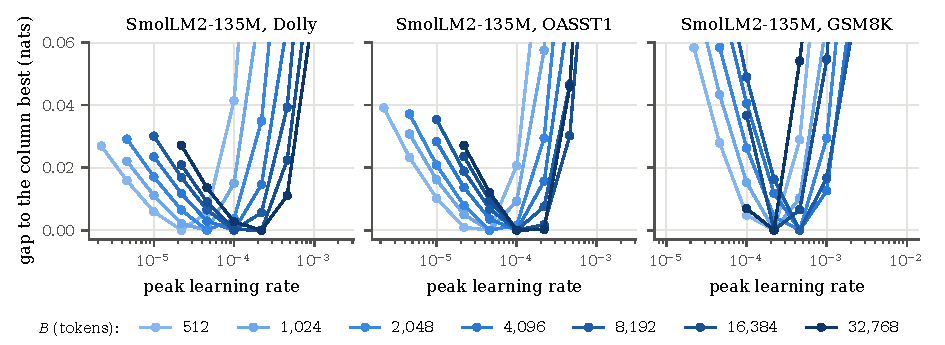
\includegraphics[width=\textwidth]{figures/lr_curves.pdf}
\caption{Seed-averaged held-out loss against peak learning rate for every batch size of the three SmolLM2-135M grids, relative to the best point of each column. Points more than 0.06 nats above the best are outside the plotted range. The curves are much steeper above the optimum than below it, and on GSM8K the optimum moves back to lower learning rates at the largest batch sizes.}
\label{fig:lrcurves}
\end{figure}

\end{document}
